% \documentclass{report}
% \usepackage[utf8]{inputenc}
% \usepackage[brazil]{babel}

\documentclass[oneside,a4paper,12pt]{normas-utf-tex}

\usepackage{breakurl}
\usepackage[alf,abnt-emphasize=bf,bibjustif,recuo=0cm, abnt-etal-cite=2]{abntcite}
\usepackage[brazil]{babel}
\usepackage[utf8]{inputenc}
\usepackage{amsmath}
\usepackage{graphicx,subfig}
\usepackage{times}
\usepackage[plain]{fancyref}
\usepackage{float}
\usepackage{pdfpages}
\usepackage{enumitem}
\usepackage{longtable}
\usepackage{amssymb}
\usepackage{empheq}
%\usepackage[loose]{units}

\newcommand{\unit}[1]{\ensuremath{\, \mathrm{~[#1]}}}



%%% Complemento para tabelas
\usepackage{booktabs, multirow}
\setlength{\heavyrulewidth}{0.1em}
\renewcommand{\toprule}{\midrule[\heavyrulewidth]}
\renewcommand{\arraystretch}{1.2}
%%%

\instituicao{Universidade Tecnológica Federal do Paraná}
\departamento{Departamento Acadêmico de Eletrônica}
\departamentodois{Departamento Acadêmico de Informática}
\programa{Curso de Engenharia de Computação}
\unidade{Oficina de Integração 3}

\titulo{\MakeUppercase{Mapeamento de ambientes com o robô Bellator}}
\documento{Terceiro entregável}

\autor{Luis Guilherme Machado Camargo}
\autordois{Pedro Alberto de Borba}
\autortres{Ricardo Farah}
\autorquatro{Stefan Campana Fuchs}
\autorcinco{Telmo Friesen}

\cita{CAMARGO, L.G.M; BORBA, P.A.; FARAH, R.; FUCHS, S.C.; FRIESEN, T}

\comentario{\UTFPRdocumentodata\ apresentado à Unidade Curricular de \UTFPRunidadedata\ do \UTFPRprogramadata\ da \ABNTinstituicaodata\ como requisito parcial para aprovação.}

\local{Curitiba}
\data{\the\year}

\begin{document}

\capa
\folhaderosto
\sumario
\chapter{Terceiro entregável - 10/04/2013}

Conforme estabelecido na relação de \textit{deliverables} do documento de análise tecnológica, este terceiro entregável consiste nos seguintes itens:
\begin{enumerate}[topsep=0pt, partopsep=0pt, itemsep=0pt]
      \item Diagramas de casos de uso e de classes (estação base).
      \item Diagrama de casos de uso (software embarcado).
      \item Diagrama de fluxo de dados (software embarcado).
      \item Diagrama em blocos (hardware).
      \item Explicação detalhada de cada bloco (hardware).
      \item Diagrama elétrico/eletrônico (hardware).
\end{enumerate}

\vspace{12pt}

Além dos itens obrigatórios dos entregáveis, estão presentes neste documento os seguintes adicionais:
\begin{enumerate}
	\item Requisitos funcionais.
	\item Descrição das classes da estação base.
	\item Diagrama de classes do sistema embarcado.
	\item Descrição das classes do sistema embarcado.
	\item Diagramas de estados.
	\item Diagramas de sequência.
	\item Diagrama em blocos do hardware.
	\item Diagrama elétrico/eletrônico do hardware.
\end{enumerate}

\chapter{Modelagem UML}

\section{Requisitos funcionais}

\begin{enumerate}[topsep=0pt, partopsep=0pt, itemsep=0pt]
%  \item A estação base deve receber informações de posicionamento do robô, processá-las e armazená-las na memória. Representado pelo requisito funcional: \textbf{``Estação base mostra na interface gráfica a posição do robô - RF\arabic{enumi}"}
%  \item A estação base deve receber informações de obstáculos detectados, processá-las e armazená-las na memória. Representado pelo requisito funcional: \textbf{"Estação base mostra na interface gráfica os novos obstáculos detectados pelo robô - RF\arabic{enumi}"}
  \item A estação base deve mostrar na interface gráfica um mapa 2D (atualizado automaticamente) representando o robô e os obstáculos detectados por ele. Representado pelo requisito funcional: \textbf{``Estação base mostra mapa 2D do robô e dos obstáculos detectados -- RF\arabic{enumi}''}.
  \item O usuátio pode salvar o mapa 2D no disco rígido. Representado pelo requisito funcional: \textbf{``O usuário pode salvar o mapa -- RF\arabic{enumi}''}.
  \item O usuário pode carregar o mapa 2D do disco rígido. Representado pelo requisito funcional: \textbf{``O usuário pode carregar o mapa -- RF\arabic{enumi}''}.
  \item A estação base deve mostrar na interface gráfica a imagem captada pela \textit{webcam} do robô. Representado pelo requisito funcional: \textbf{``Estação base mostra a imagem captada pela webcam -- RF\arabic{enumi}''}.
  \item O usuário pode movimentar o robô, controlando a velocidade de suas rodas remotamente pelo teclado da estação base. Representado pelo requisito funcional: \textbf{``O usuário pode movimentar o robô -- RF\arabic{enumi}''}.
  \item A estação base deve ser capaz de estabelecer conexão com o robô, informando o usuário caso a conexão ocorra com sucesso ou não. Representado pelo requisito funcional \textbf{``O usuário pode estabelecer a conexão entre o robô e a estação base -- RF\arabic{enumi}''}.
\end{enumerate}

\section{Requisitos não funcionais}

\begin{enumerate}[topsep=0pt, partopsep=0pt, itemsep=0pt]
  \item A imagem transmitida pela câmera do robô deve ser colorida. Representado pelo requisito não funcional: \textbf{``O robô deve enviar vídeo em imagem colorida para a estação base - RNF\arabic{enumi}''}.
  \item O robô deve transmitir as imagens de sua câmera em tempo real. Representado pelo requisito não funcional: \textbf{``O robô deve transmitir os dados de vídeo captados pela câmera em tempo real - RNF\arabic{enumi}''}.
%  \item O método de entrada do usuário deve se dar por meio de interface gráfica com o auxílio do mouse. Representado pelo requisito não funcional: \textbf{"O usuário pode interagir com o robô por meio do mouse - RNF0\arabic{enumi}"}.
%  \item O método de entrada do usuário deve se dar por meio de interface gráfica com o auxílio do teclado. Representado pelo requisito não funcional: \textbf{"O usuário pode interagir com o robô por meio do teclado - RNF0\arabic{enumi}"}.
\end{enumerate}


\section{Casos de uso identificados}

\begin{enumerate}[topsep=0pt, partopsep=0pt, itemsep=0pt]
  \item Visualização de mapa 2D na interface gráfica segundo os dados lidos dos sensores do robô. Representado pelo caso de uso: \textbf{``Mostrar mapa - UC\arabic{enumi}''}.
  \item Gravação do mapa em um arquivo no disco rígido. Representado pelo caso de uso: \textbf{``Salvar mapa - UC\arabic{enumi}''}. 
  \item Leitura do mapa de um arquivo do disco rígido. Representado pelo caso de uso: \textbf{``Carregar mapa - UC\arabic{enumi}''}.
  \item Leitura de informações dos sensores do robô. Representado pelo caso de uso: \textbf{``Ler amostras dos sensores - UC\arabic{enumi}''}.
  \item Visualização de imagens da \textit{webcam} do robô. Representado pelo caso de uso: \textbf{``Visualizar imagens da câmera - UC\arabic{enumi}''}.
  \item Alteração pelo usuário da velocidade das rodas do robô. Representado pelo caso de uso: \textbf{``Alterar velocidade das rodas - UC\arabic{enumi}''}.
  \item Solicitação de estabelecimento de conexão com o robô. \textbf{``Estabelecer conexão - UC\arabic{enumi}''}.
%  \item Inclusão de novos obstáculos e suas posições lidos do robô. Representado pelo caso de uso: \textbf{``Mostrar posição dos novos obstáculos detectados na tela - UC\arabic{enumi}''}.
  \item Consulta à documentação do robô pelo usuário. Representado pelo caso de uso: \textbf{``Consultar documentação do robô - UC\arabic{enumi}''}.
\end{enumerate}

Foram produzidos três Diagramas de Casos de Uso (Figuras \ref{fig:diagrama_caso_uso_estacao_base}, \ref{fig:diagrama_caso_uso_linux_embarcado} e \ref{fig:diagrama_caso_uso_placa_embarcada}) com base nos casos de uso apresentados. O primeiro diagrama representa o \textit{software} da estação base, e o segundo e o terceiro representam o sistema embarcado (TS-7260 e placa de baixo nível, respectivamente).

\begin{figure}[H]
  \centering
  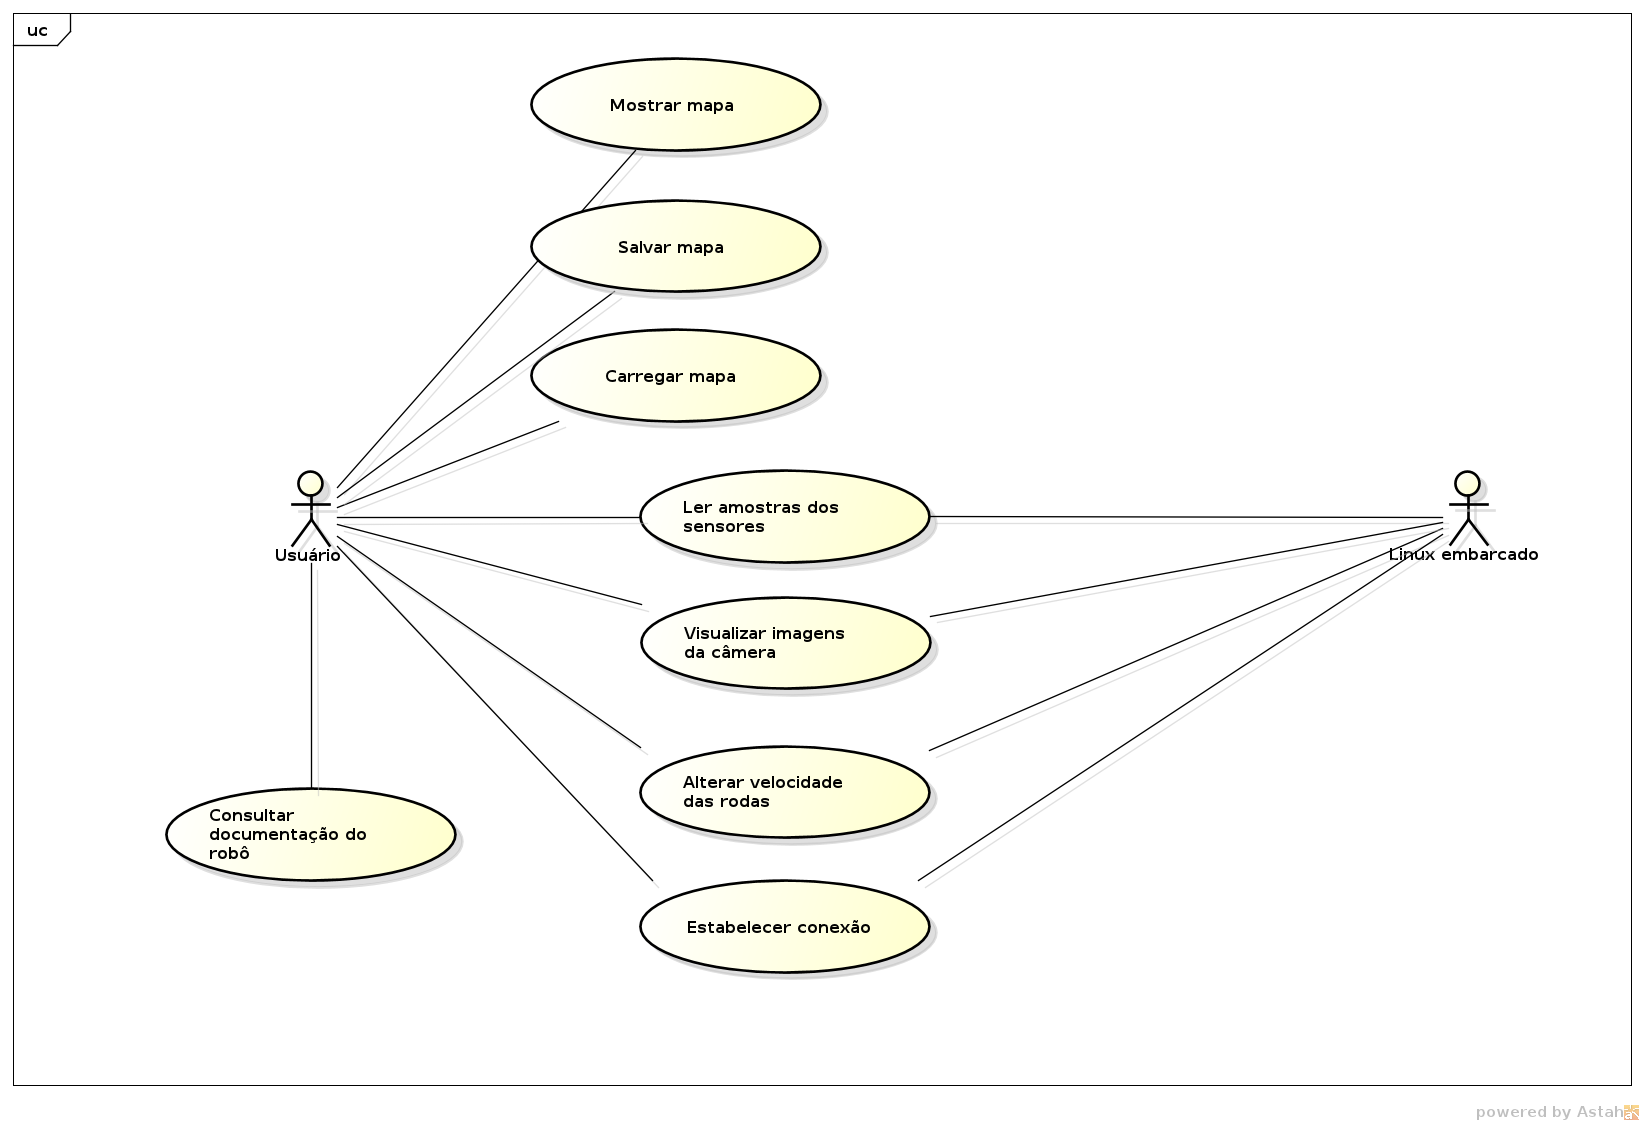
\includegraphics[width=\textwidth, keepaspectratio]{./figuras/diagrama_caso_uso_estacao_base.png}
  \caption{Diagrama de casos de uso do \textit{software} da estação base.}
  \label{fig:diagrama_caso_uso_estacao_base}
\end{figure}

\begin{figure}[H]
  \centering
  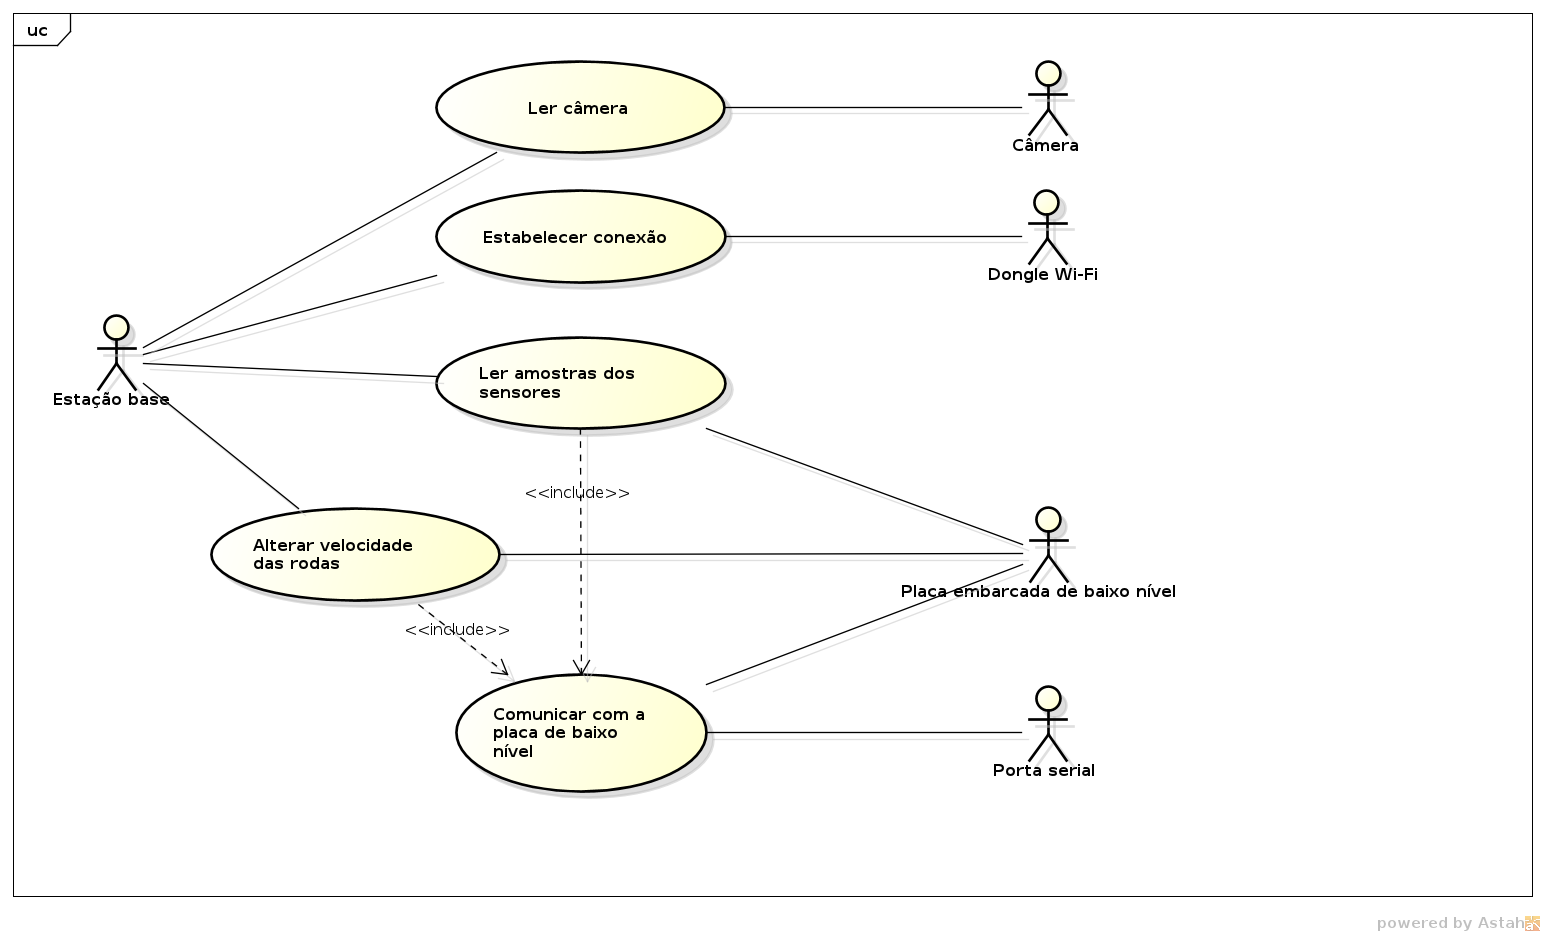
\includegraphics[width=\textwidth, keepaspectratio]{./figuras/diagrama_caso_uso_linux_embarcado.png}
  \caption{Diagrama de casos de uso do \textit{software} para a placa TS-7260.}
  \label{fig:diagrama_caso_uso_linux_embarcado}
\end{figure}

\begin{figure}[H]
  \centering
  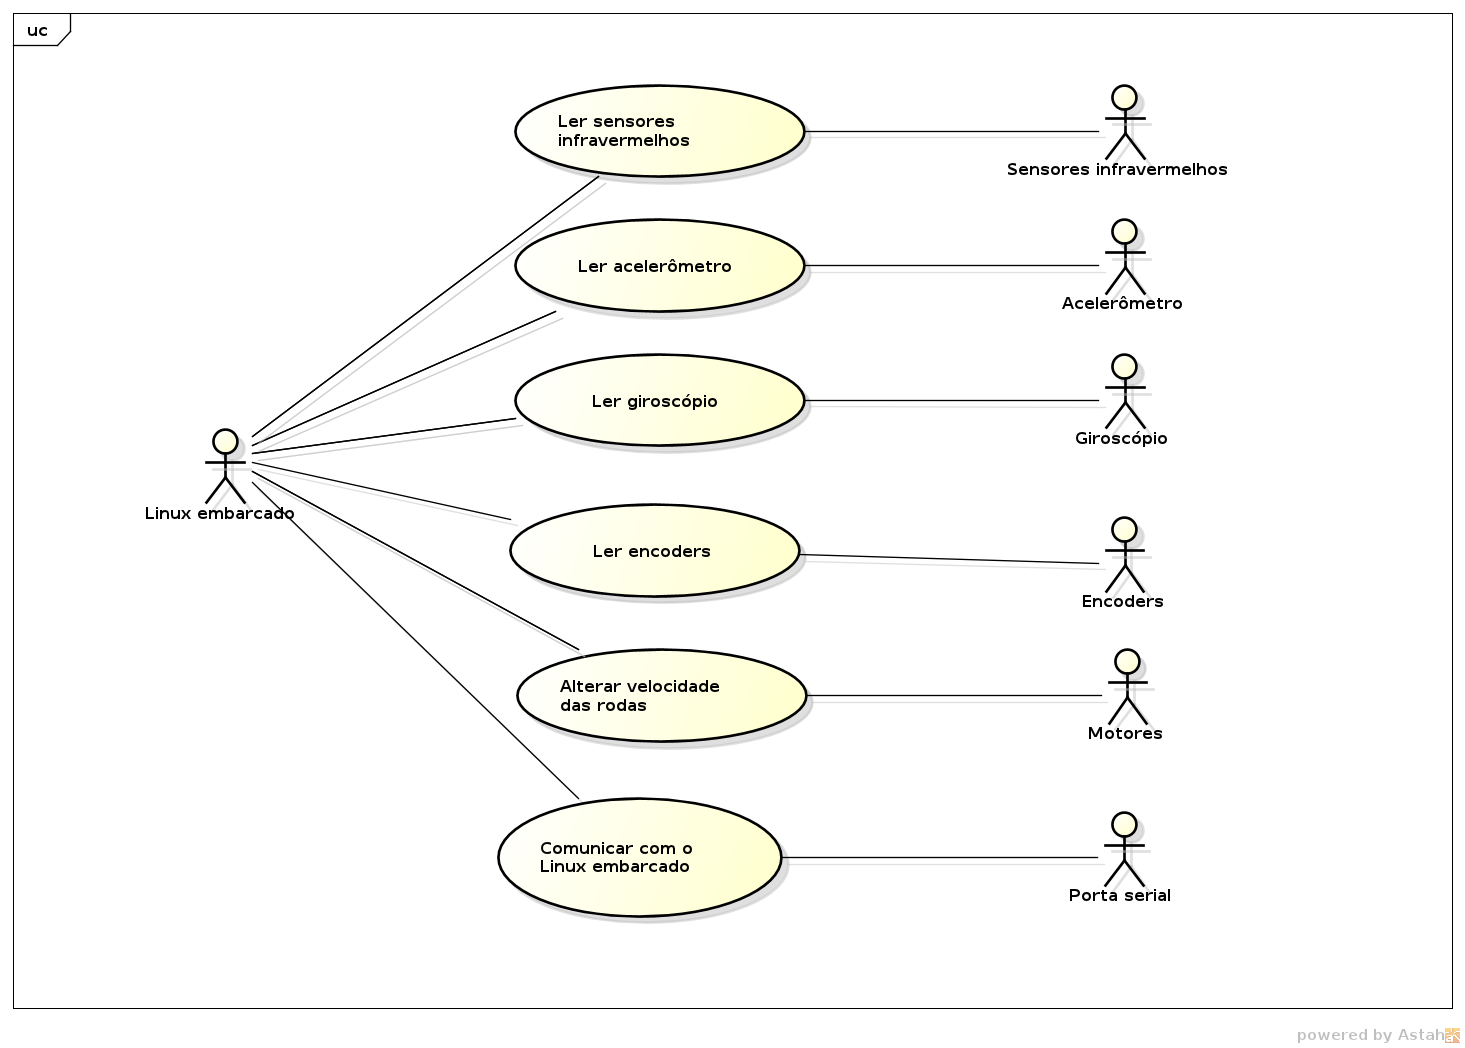
\includegraphics[width=\textwidth, keepaspectratio]{./figuras/diagrama_caso_uso_placa_embarcada.png}
  \caption{Diagrama de casos de uso do \textit{software} para a placa de baixo nível.}
  \label{fig:diagrama_caso_uso_placa_embarcada}
\end{figure}

\section{Diagrama de classes da estação base}

A Figura \ref{fig:diagrama_classes_estacao_base} mostra o diagrama de classes da estação base.
\begin{figure}[H]
  \centering
  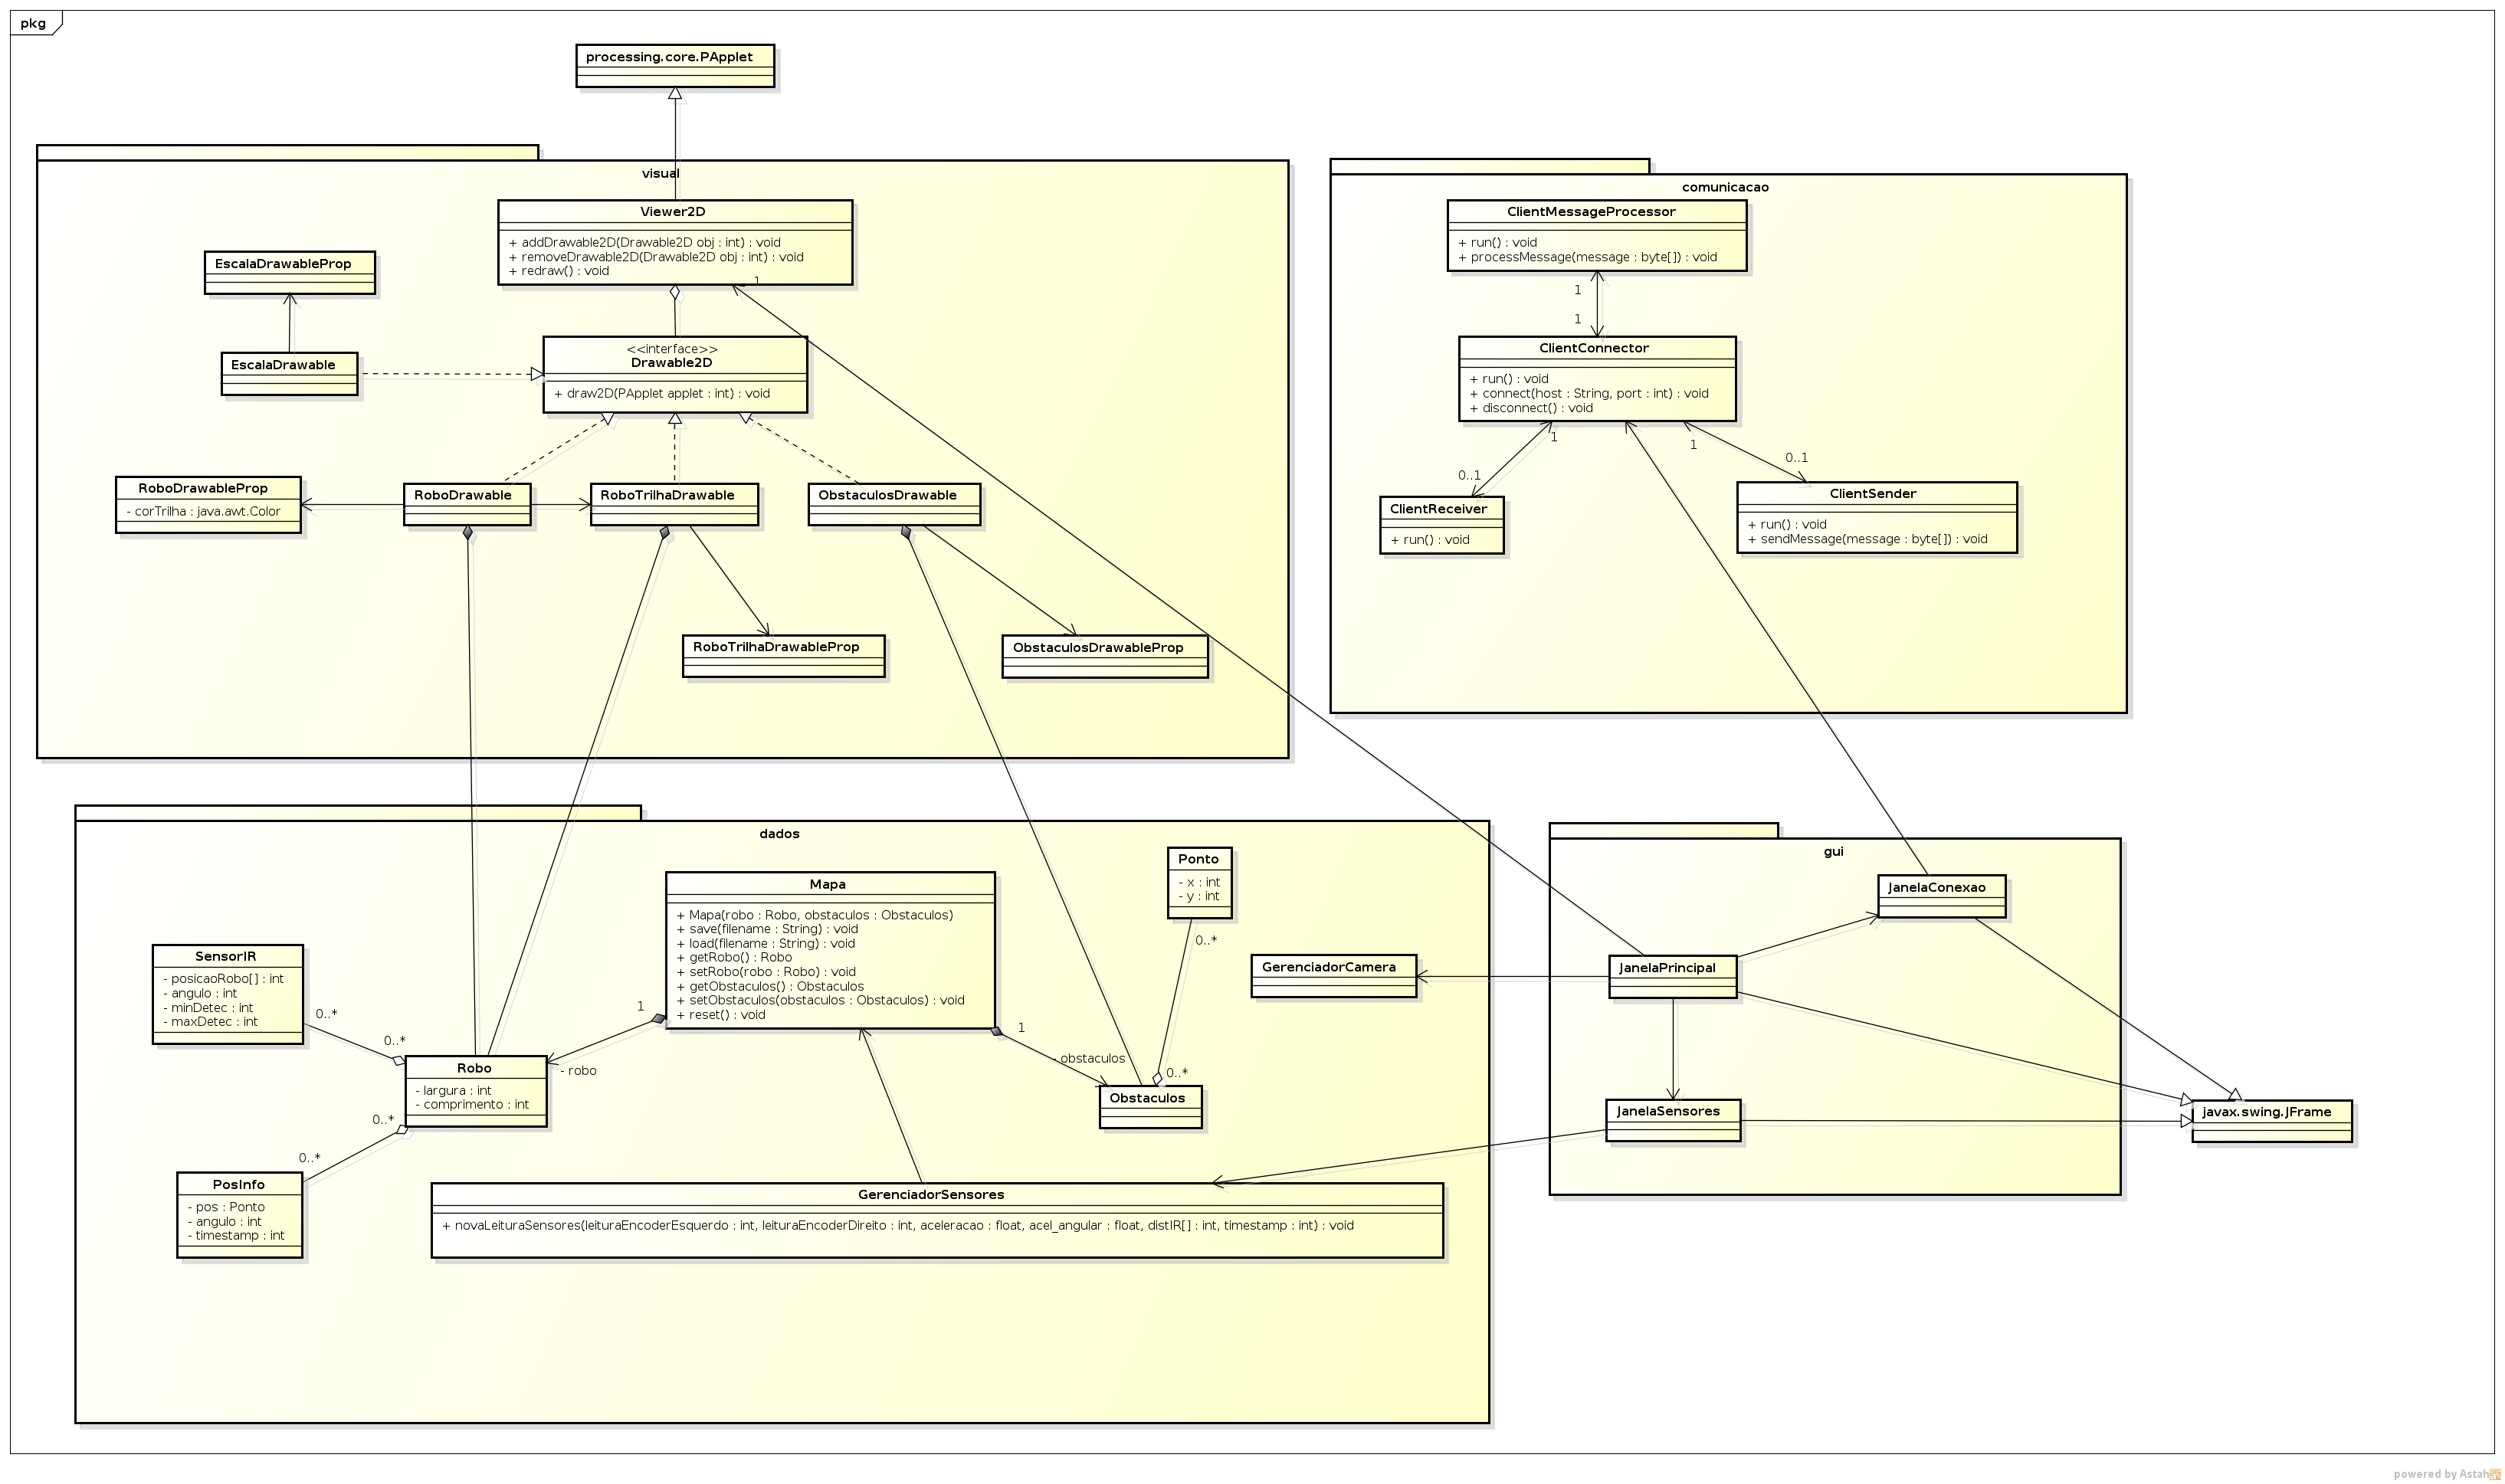
\includegraphics[width=\textwidth]{./figuras/diagrama_classes_estacao_base.png}
  \caption{Diagrama de classes da estação base}
  \label{fig:diagrama_classes_estacao_base}
\end{figure}

\subsection{Descrição das classes da estação base}
%O software da estação base do robô foi dividido em cinco pacotes:  visual, controle, comunicação, controle.robo e interface gráfica. Estes serão descritos com suas respectivas classes na Tabela \ref{tab:pacote_visual}.
O \textit{software} da estação base do robô foi dividido em cinco pacotes:  \textit{visual}, \textit{dados}, \textit{comunicao}, e \textit{gui}. A seguir há uma descrição de cada pacote e das suas respectivas classes.


\subsection{Pacote \textit{visual}}

Este pacote consiste de toda a parte visual da estação base e conta com as seguintes classes: Viewer2D, Drawable2D, EscalaDrawable, RoboDrawable, RoboTrilhaDrawable, ObstaculosDrawable, EscalaDrawableProp, RoboDrawableProp, RoboTrilhaDrawableProp e ObstaculosDrawableProp. Na Tabela \ref{tab:pacote_visual} estão descritas as classes deste pacote.


\begin{table}[h]
  \centering
  \caption{Pacote \textit{visual}}
  \begin{tabular}{p{6cm}p{8cm}}
    \toprule
    \textbf{Classe} & \textbf{Descrição} \\
    \midrule
    Viewer2D & Responsável por exibir os objetos Drawable2D. Possui recursos de pan, zoom e rotate.   \\ \hline
    Drawable2D & Representa genericamente objetos 2D que podem ser desenhados em um Viewer2D. \\ \hline
    EscalaDrawable & Responsável por desenhar uma escala gráfica no mapa. \\ \hline
    RoboDrawable & Responsável por desenhar o robô no mapa. \\ \hline
    RoboTrilhaDrawable & Responsável por desenhar a trilha percorrida pelo robô no mapa. \\ \hline
    ObstaculosDrawable & Responsável por desenhar os pontos de cada obstáculo no mapa. \\ \hline
    EscalaDrawableProp & Contém as propriedades visuais de desenho da escala. \\ \hline
    RoboDrawableProp & Contém as propriedades visuais de desenho do robô \\ \hline
    RoboTrilhaDrawableProp & Contém as propriedades visuais de desenho da trilha do robô. \\ \hline
    ObstaculosDrawableProp & Contém as propriedades visuais de desenho dos obstáculos. \\
    \bottomrule
  \end{tabular}%
  \label{tab:pacote_visual}%
\end{table}%

\subsection{Pacote \textit{dados}}

Este pacote consiste de toda a parte da estação base que processa e armazena as informações essenciais do robô e do mapa. Conta com as seguintes classes: Mapa, Obstaculos, Robo, ControleSensores, Posinfo, SensorIR e Ponto. Na Tabela \ref{tab:pacote_controle} estão descritas as classes deste pacote.

\begin{table}[h]
  \centering
  \caption{Pacote \textit{dados}}
  \begin{tabular}{p{6cm}p{8cm}}
    \toprule
    \textbf{Classe} & \textbf{Descrição} \\ 
    \midrule
    Mapa  & Responsável por representar o mapa. Armazena as informações essenciais do robô e dos obstáculos detectados. \\ \hline
    Obstaculos & Responsável por conter os obstáculos detectados pelo robô. \\ \hline
    Robo  & Responsável por representar o robô, este contêm largura, comprimento e centro de movimento (ponto central entre as duas rodas). \\ \hline
    GerenciadorSensores & Responsável por atualizar a posição do robô e dos pontos que representam os obstáculos, de acordo com as leituras feitas pelos sensores. \\ \hline
    Posinfo & Responsável por conter as informações de uma posição do robô. \\ \hline
    SensorIR & Responsável por representar um sensor IR do robô. \\ \hline 
    Ponto & Representa um ponto de cordenadas cartesianas (x,y). \\ \hline
    GerenciadorCamera & Responsável por gerenciar o status da câmera e o recebimento de imagens. \\ 
    \bottomrule
  \end{tabular}%
  \label{tab:pacote_controle}%
\end{table}%

\subsection{Pacote \textit{comunicacao}}
\label{subsec:pacote_comunicacao}

%Este pacote consiste em toda a parte de comunicação da estação base com o robô e conta com as seguintes classes: ClientCommandInterpreter, ClientConnection, ClientReceiver, ClientSender, ServerCommandInterpreter, ServerListener, ServerSender, ServerReceiver e Message. Na Tabela \ref{tab:pacote_comunicacao} estão descritas as classe deste pacote.
Este pacote consiste em toda a parte de comunicação da estação base com o robô e conta com as seguintes classes: ClientMessageProcessor ClientConnection, ClientReceiver, ClientSender e Message. Na Tabela \ref{tab:pacote_comunicacao} estão descritas as classes deste pacote.

É importante ressaltar que o protocolo TCP requer obrigatoriamente a especificação de um cliente e de um servidor para estabelecimento de uma conexão. Nas implementações desse protocolo em diversas linguagens (como Java e C++) existem tipos de \textit{socket} distintos para cliente e servidor. Na criação de um \textit{socket} de servidor, há obrigatoriamente a atribuição de uma porta de escuta, na qual o servidor aguarda que um cliente efetue uma requisição de conexão. Não é possível, ao menos nas implementações atuais do TCP, estabelecer conexão entre dois \textit{sockets} de cliente ou entre dois \textit{sockets} de servidor. Como neste projeto, o robô proverá serviços à estação base (envio de imagens da câmera, envio de leituras de sensores, além de prover a posibilidade de comando dos motores) o robô foi escolhido como servidor e a estação base como cliente. Enfatiza-se que o paradigma cliente-servidor não implica de forma alguma que a comunicação seja unidirecional. Pelo contrário, o envio de pacotes 
pode ser feito bidirecionalmente após uma conexão TCP ser estabelecida, sem nenhuma restrição quanto a isso.

\begin{table}[h]
  \centering
  \caption{Pacote \textit{comunicacao}}
  \begin{tabular}{p{6cm}p{8cm}}
    \toprule
    \textbf{Classe} & \textbf{Descrição} \\ 
    \midrule
    ClientMessageProcessor & Thread responsável pelo processamento de mensagens recebidas de um host de conexão. \\ \hline
    ClientConnector & Thread responsável por efetuar a gerência da conexão do cliente (estação base) com o servidor (robô). \\ \hline
    ClientReceiver & Thread responsável por receber mensagens de um host de uma conexão. \\ \hline
    ClientSender & Thread responsável por enviar mensagens ao host de uma conexão. \\ \hline
%    ServerCommandInterpreter & Responsável pela interpretação dos comandos do servidor. Os comandos recebidos são inseridos em uma fila, de modo a serem posteriormente executados pela thread. \\ \hline
%    Server & Responsável gerenciar o servidor (robô). \\ \hline
%    ServerListener & Responsável por escutar as novas conexões de clientes. \\ \hline
%    ServerSender & Responsável por enviar mensagens ao host de uma conexão. \\ \hline
%    ServerReceiver & Responsável por receber mensagens de um host de uma conexão. \\ \hline
%     Message & Contém uma mensagem a ser enviada por um Sender. \\ 
    \bottomrule
  \end{tabular}%
  \label{tab:pacote_comunicacao}%
\end{table}%

\subsection{Pacote \textit{gui}}

Este pacote consiste em toda a interface gráfica do sistema e conta com as seguintes classes: JanelaConexao, JanelaPrincipal e JanelaSensores. Na Tabela \ref{tab:pacote_interface_grafica} estão descritas as classes deste pacote.

\begin{table}[h]
  \centering
  \caption{Pacote \textit{gui}}
  \begin{tabular}{p{6cm}p{8cm}}
    \toprule
    \textbf{Classe} & \textbf{Descrição} \\ 
    \midrule
    JanelaConexao & Janela com as informações e configurações da conexão com o Bellator. \\ \hline
    JanelaPrincipal & Janela principal da interface gráfica da estação base. \\ \hline
    JanelaSensores & Janela de configuração dos sensores. \\ 
    \bottomrule
  \end{tabular}%
  \label{tab:pacote_interface_grafica}%
\end{table}%

\section{Fluxo de dados}

A Figura \ref{fig:diagrama_fluxo_dados} mostra o diagrama de fluxo de dados.

\begin{figure}[H]
  \centering
  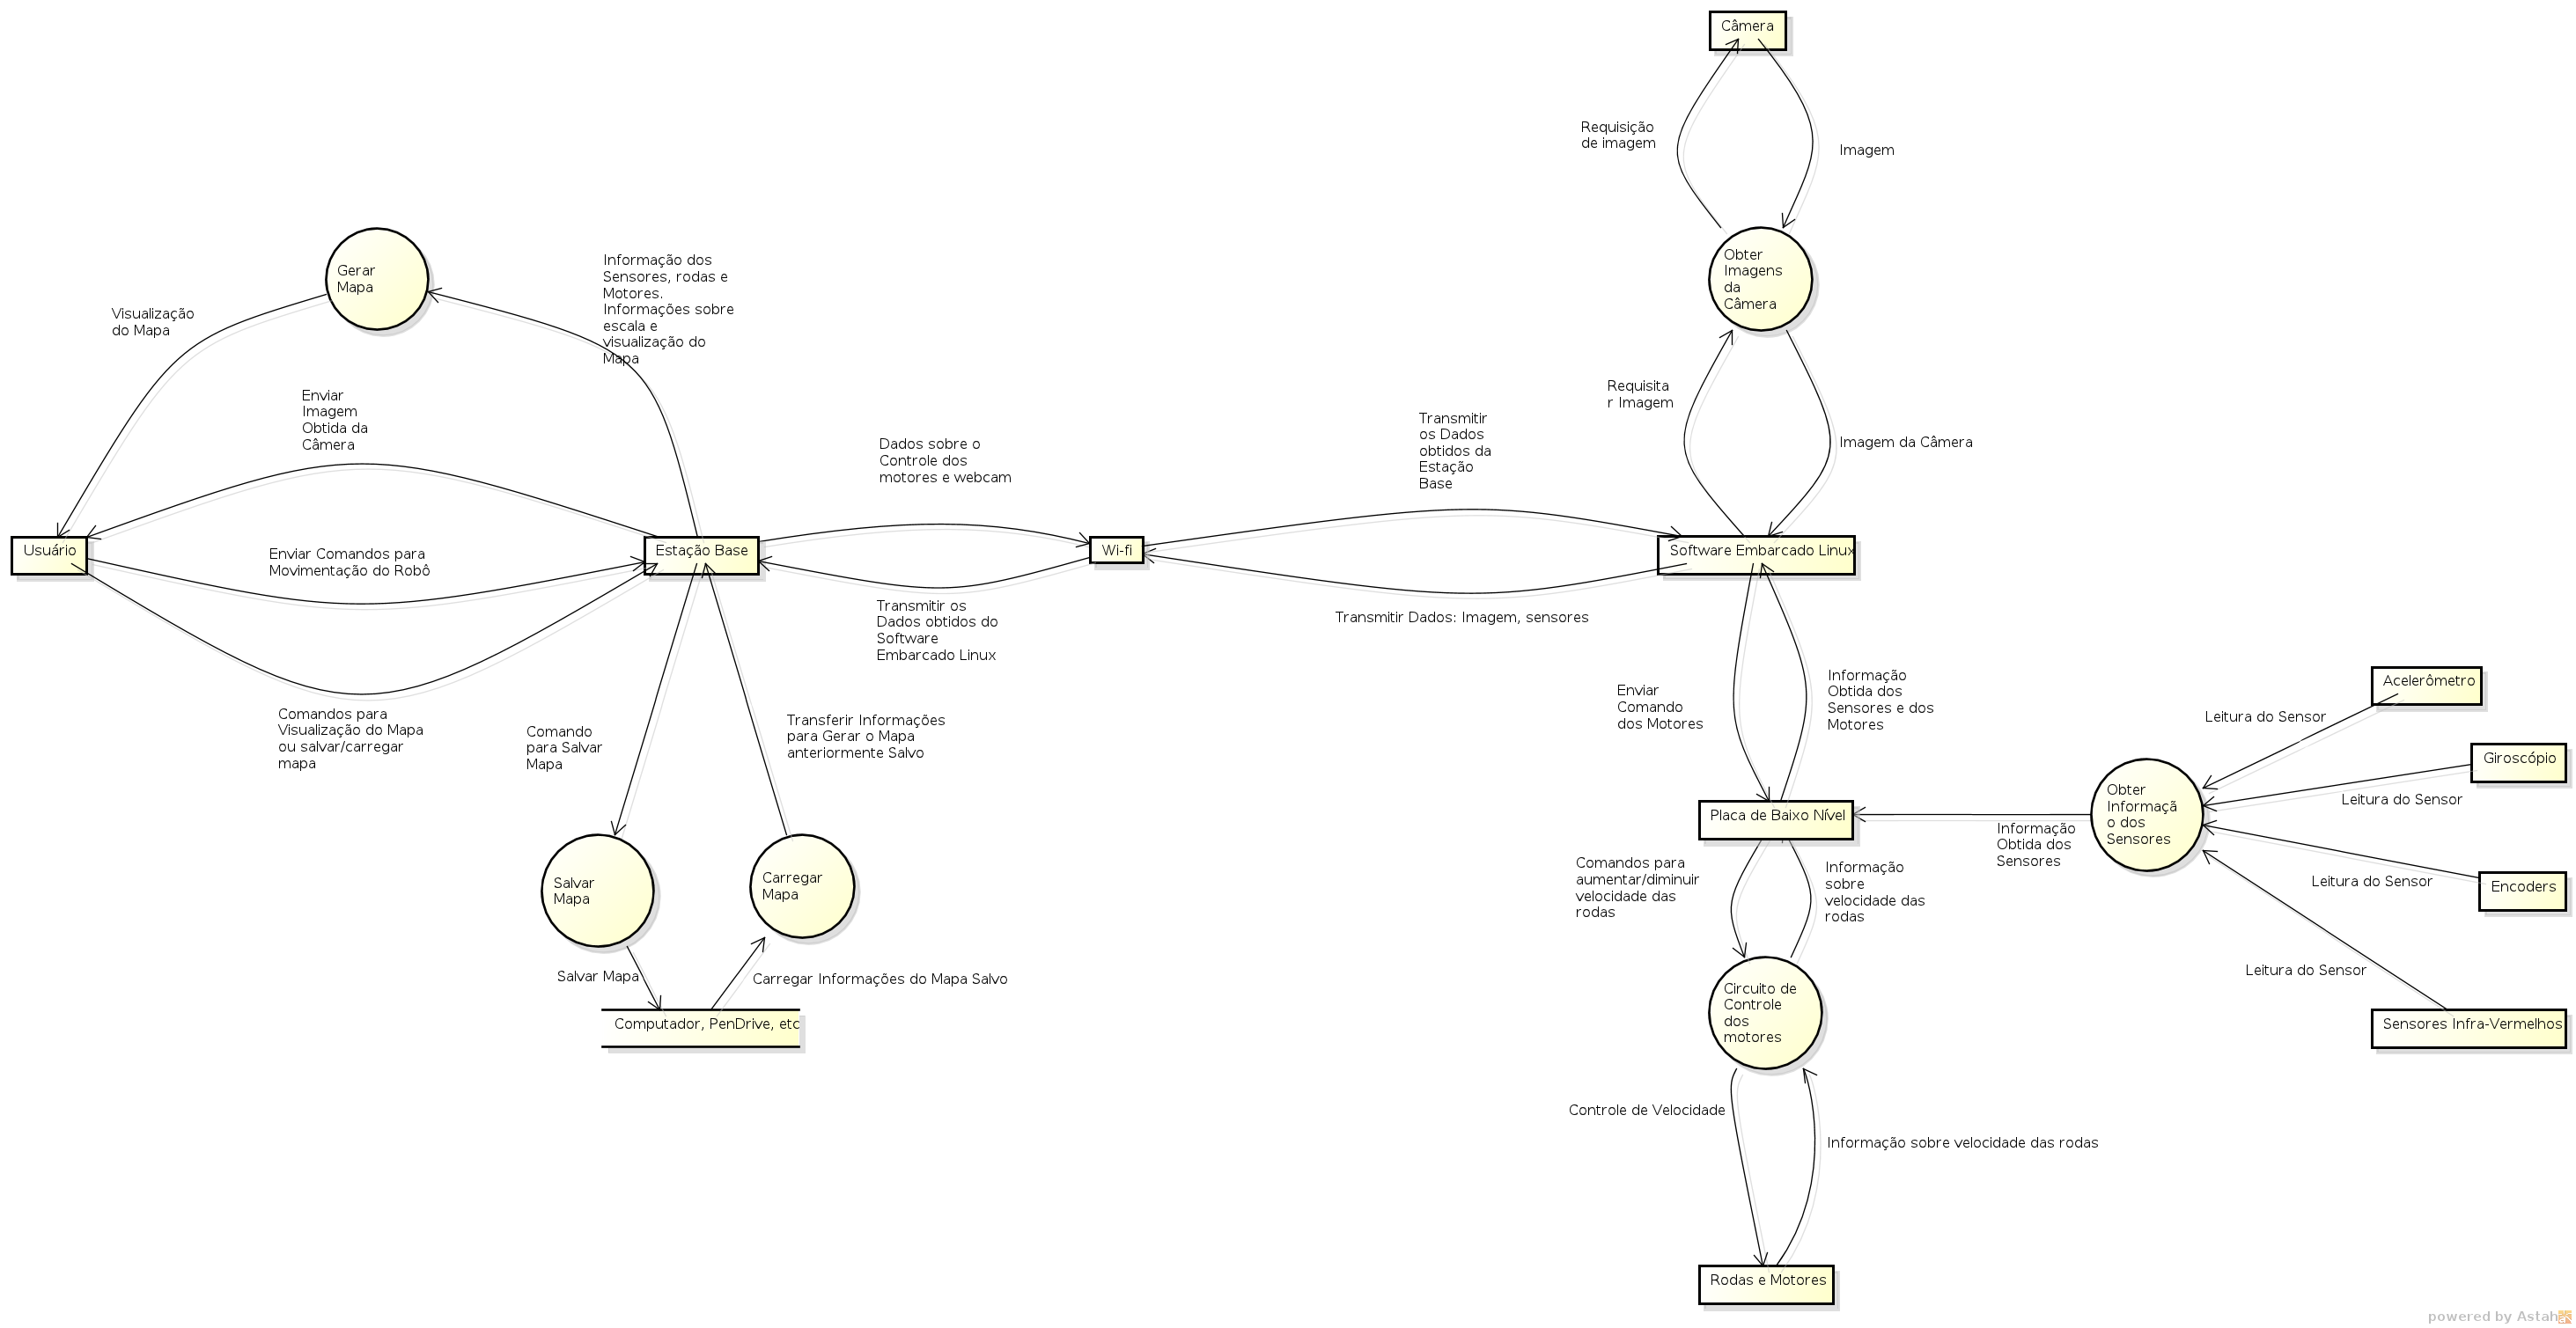
\includegraphics[width=\textwidth, keepaspectratio]{./figuras/diagrama_fluxo_dados.png}
  \caption{Diagrama de fluxo de dados.}
  \label{fig:diagrama_fluxo_dados}
\end{figure}

% \section{Diagrama de estados}
% As Figuras \ref{fig:diagrama_estados_estacao_base} e \label{fig:diagrama_estados_sistema_embarcado} mostram os diagramas de estados do sistema.
% 
% \begin{figure}[H]
%   \centering
%   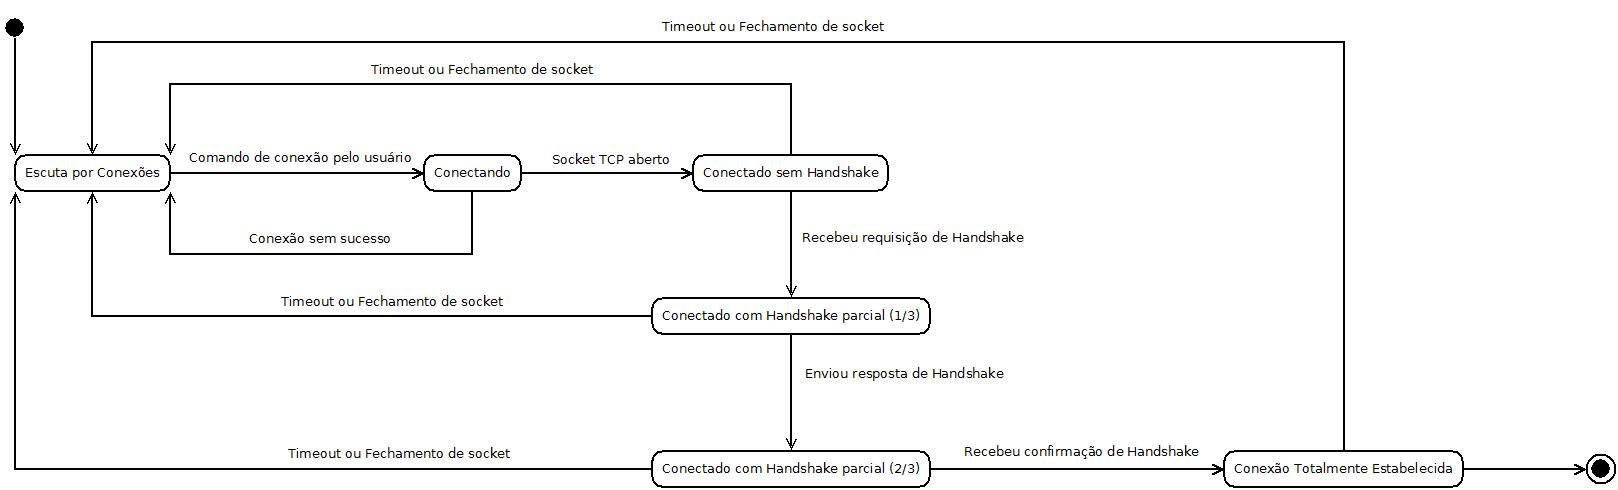
\includegraphics[width=\textwidth, keepaspectratio]{./figuras/diagrama_estados_estacao_base.jpeg}
%   \caption{Diagrama de estados para a estação base.}
%   \label{fig:diagrama_estados_estacao_base}
% \end{figure}
% 
% \begin{figure}[H]
%   \centering
%   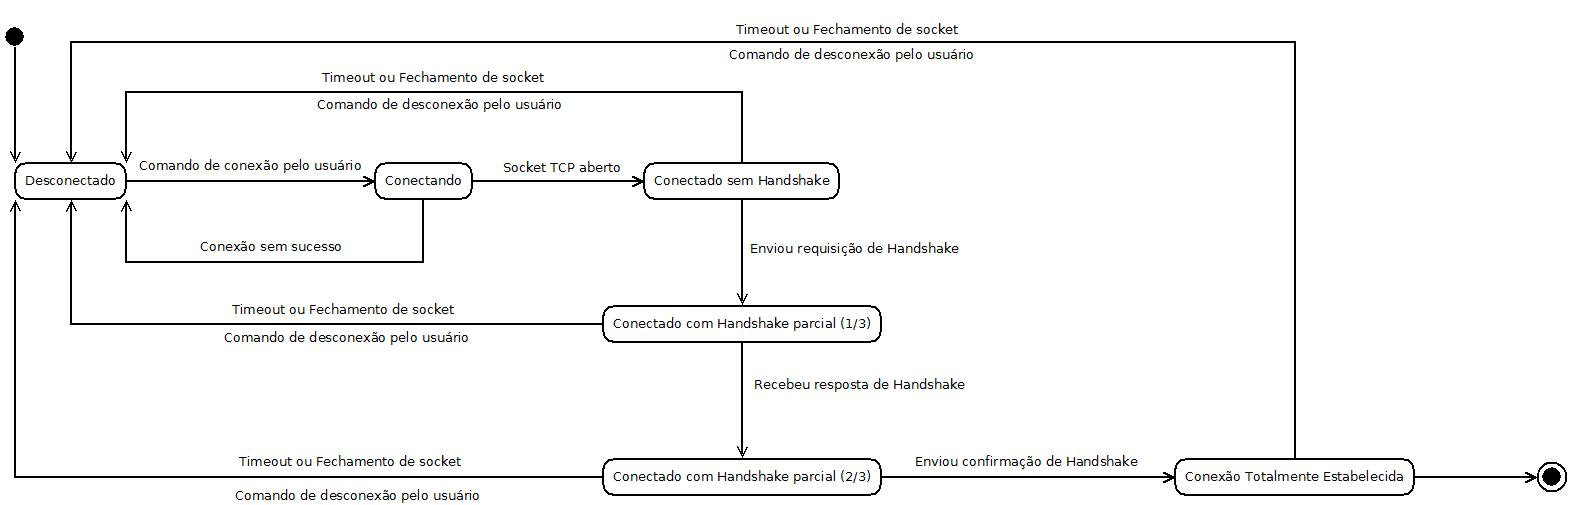
\includegraphics[width=\textwidth, keepaspectratio]{./figuras/diagrama_estados_sistema_embarcado.jpeg}
%   \caption{Diagrama de estados para o sistema embarcado.}
%   \label{fig:diagrama_estados_sistema_embarcado}
% \end{figure}


\section{Diagrama de classes do sistema embarcado}


A Figura \ref{fig:diagrama_classes_sist_embarcado} mostra o diagrama de classes do sistema embarcado (placa TS-7260).
\begin{figure}[H]
  \centering
  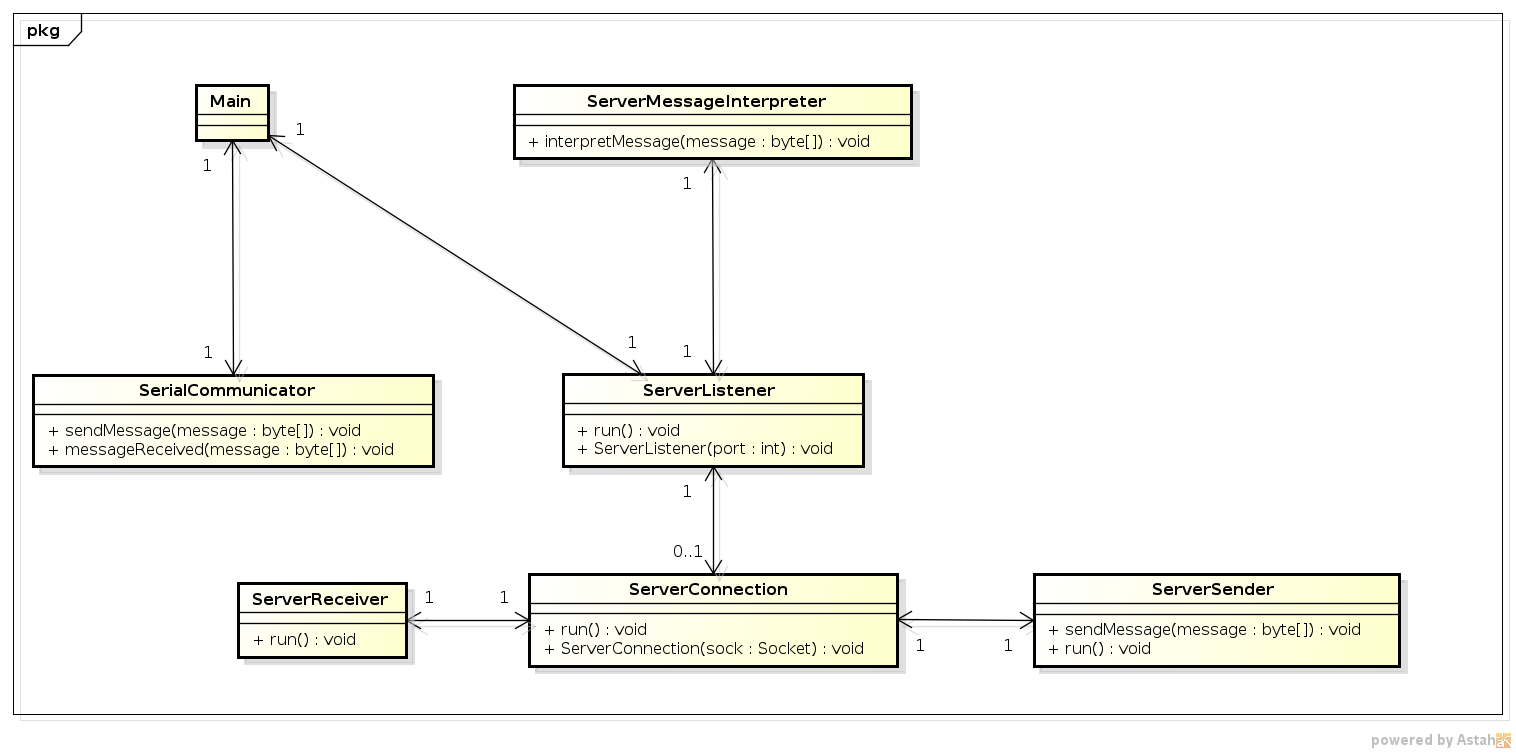
\includegraphics[width=\textwidth]{./figuras/diagrama_classes_sist_embarcado.png}
  \caption{Diagrama de classes do sistema embarcado (placa TS-7260).}
  \label{fig:diagrama_classes_sist_embarcado}
\end{figure}



%\subsection{Descrição das classes do sistema embarcado (TS-7260)}

\begin{table}[h]
  \centering
  \caption{Descrição das classes do sistema embarcado (placa TS-7260)}
  \begin{tabular}{p{6cm}p{8cm}}
    \toprule
    \textbf{Classe} & \textbf{Descrição} \\ 
    \midrule
   Main & Classe principal do robô. \\ \hline
   SensorsSampler & Thread responsável por requisitar amostras dos sensores da plca de baixo nível em intervalos de tempo previamente programados. \\ \hline
   ServerMessageProcessor & Thread responsável por realizar o processamento de mensagens recebidas de um host de conexão. \\ \hline
   ServerListener & Thread responsável por escutar requisições de conexão. \\ \hline
   ServerSender & Thread responsável por enviar mensagens ao host de uma conexão. \\ \hline
   ServerReceiver & Thread responsável por receber mensagens de um host de uma conexão. \\ \hline
   SerialCommunicator & Responsável por gerenciar a comunicação via porta serial entre a TS-7260 e a LPC2103.\\
    \bottomrule
  \end{tabular}%
  \label{tab:pacote_comunicacao}%
\end{table}%



\section{Protocolo de comunicação}

Esta seção detalha o protocolo de comunicação estabelecido entre a estação base, a placa TS-7260 (sistema com linux embarcado) e a placa LPC2103 (sistema embarcado de baixo nível).

O protocolo desenvolvido para a comunicação (via Wi-Fi) entre a estação base e a TS-7260 visa utilizar o TCP como camada de transporte. Como foi explicitado anteriormente na seção \ref{subsec:pacote_comunicacao}, o robô foi escolhido como servidor da conexão, e a estação base como cliente. Para haver confirmação da conexão entre os dois, optou-se por criar um protocolo de \textit{handshake} semelhante ao existente no TCP, de 3 passos: requisição, resposta, confirmação. A requisição é feita pelo cliente no início da conexão, a resposta é dada pelo servidor em seguida. Posteriormente, o cliente envia uma mensagem de confirmação, e a conexão é totalmente estabelecida. O uso do \textit{handshake} contribui para tanto a estação base como o sistema embarcado confirmarem que estão conectados um ao outro e não a um servidor/cliente qualquer.

Para possibilitar que o tráfego de mensagens possa ser feito de forma rápida, reduzindo atrasos, o envio e recebimento de mensagens é feito de forma assíncrona.
Essa escolha foi feita tendo em vista que, em uma comunicação totalmente síncrona, um programa (ou thread) é bloqueado ao chamar uma função de recebimento ou envio, até que efetivamente seja completa a transação. Supondo que só houvesse uma thread gerenciando a conexão, o programa não poderia enviar ou receber dados ao mesmo tempo em \textit{full-duplex}, mas somente \textit{half-duplex} (somente enviar ou somente receber).

A solução desenvolvida para possibilitar a comunicação assíncrona foi o uso de 4 threads (tanto na estação base quanto no sistema embarcado) para gerenciar os diversos aspectos envolvidos nela. A primeira \textit{thread} (a gerenciadora principal de conexão) é a responsável por estabelecer e manter a conexão, além de gerenciar os potenciais erros que possam ocorrer (tempo excessivo sem comunicação e fechamento de socket). Para a estação base, o diagrama de estados dessa \textit{thread} está representado na Figura \ref{fig:diagrama_estados_estacao_base}, e para o sistema embarcado na Figura \ref{fig:diagrama_estados_sist_embarcado}.

A segunda \textit{thread} tem a função de gerenciar o envio de mensagens. O programa principal, ao necessitar enviar uma mensagem, faz uma requisição a essa \textit{thread} que insere a mensagem em uma fila de envio. O programa principal não fica bloqueado, dessa forma, pois não necessita aguardar a mensagem ser completamente enviada, podendo efetuar outras tarefas. O diagrama de estados dessa \textit{thread} está presente na Figura \ref{fig:diagrama_estados_sender}.

A terceira \textit{thread} gerencia o recebimento de mensagens. Seu funcionamento é relativamente simples: ela possui um loop, no qual aguarda até alguma mensagem ser recebida. Quando ocorre o recebimento de alguma mensagem, ela é encaminhada para a quarta \textit{thread} (cuja explicação está a seguir) que processa o conteúdo dela e executa as operações que são necessárias para cada tipo de mensagem. Dessa forma, novas mensagens podem ser recebidas rapidamente, pois o receptor não fica bloqueado realizando o processamento das informações recebidas. O diagrama de estados dessa terceira \textit{thread} está presente na Figura \ref{fig:diagrama_estados_receiver}.

A quarta \textit{thread}, como já exposto, é a responsável por processar mensagens recebidas e realizar as operações que são necessárias para cada tipo de mensagem, o que depende da codificação exposta na seção \ref{sec:codificacao_mensagens}. Ela possui uma fila, na qual são inseridas as mensagens a serem processadas. Dessa forma a \textit{thread} receptora não necessita ficar bloqueada aguardando o término do processamento. O diagrama de estados dessa quarta \textit{thread} está presente na Figura \ref{fig:diagrama_estados_processor}.


\subsection{Codificação das mensagens}
\label{sec:codificacao_mensagens}

\begin{itemize}
  \item Mensagens do TS-7260 para o LPC2103 (via porta serial)
    	
	\begin{itemize}
		
	  \item \textbf{SYNC (0xA0)}\\
	  Quando o microcontrolador LPC2103 recebe esta mensagem, responde com as leituras mais recentes dos encoders, de cada sensor de distância, do acelerômetro e do giroscópio (enviando uma mensagem SENSORS, explicada abaixo).
	  
	  \item \textbf{ENGINES (0xB0)}\\
	  \textit{(byte) vel\_roda\_esquerda}\\
	  \textit{(byte) vel\_roda\_direita}\\
	  \textit{(byte) CHECKSUM\_H}\\
	  \textit{(byte) CHECKSUM\_L}\\
	  Ao receber este comando, o microcontrolador utiliza os valores para definir o nível de PWM para as rodas do robô. Os valores de velocidade são representados por um byte cada, nos quais o bit mais significativo indica o sentido de rotação da roda (1 para frente e 0 para trás) e os restantes a intensidade do PWM.
	  
	  Os bytes de checksum são utilizados para verificar se não há dados corrompidos. Os bytes da mensagem são somados (módulo 65536) e o resultado é atribuído aos bytes (high e low) de checksum.
	  \end{itemize}
	  
	  \item Mensagens do LPC2103 para a TS-7260 (via porta serial)
	  
	  \begin{itemize}

	  \item \textbf{ENGINES\_ACK (0xB1)}\\
	  \textit{(byte) vel\_roda\_esquerda}\\
	  \textit{(byte) vel\_roda\_direita}\\
	  \textit{(byte) CHECKSUM\_H}\\
	  \textit{(byte) CHECKSUM\_L}\\
	  Esta mensagem deve ser enviada toda vez que um comando de mudança de velocidade (ENGINES) for recebido na placa de baixo nível. A mensagem é usada no Linux embarcado para verificar se o comando foi corretamente recebido. Caso uma confirmação não seja recebida em certo intervalo de tempo, outro comando ENGINES é enviado para a placa de baixo nível.
	 
	  O checksum é tem função idêntica ao que já foi explicitado na mensagem ENGINES.
	  
	  \item \textbf{SENSORS (0xC0)}\\
	  \textit{(byte) encoder\_esq\_H}, \textit{(byte) encoder\_esq\_L},\\
	  \textit{(byte) encoder\_dir\_H}, \textit{(byte) encoder\_dir\_L},\\
	  \textit{(byte) IR1}, \textit{(byte) IR2}, \textit{(byte) IR3}, \textit{(byte) IR4}, \textit{(byte) IR5},\\
	  \textit{(byte) AX\_H}, \textit{(byte) AX\_L},\\
	  \textit{(byte) AY\_H}, \textit{(byte) AY\_L},\\
	  \textit{(byte) AZ\_H}, \textit{(byte) AZ\_L},\\
	  \textit{(byte) GX\_H}, \textit{(byte) GX\_L},\\
	  \textit{(byte) GY\_H}, \textit{(byte) GY\_L},\\
	  \textit{(byte) GZ\_H}, \textit{(byte) GZ\_L},\\
	  \textit{(byte) TIMESTAMP\_H}, \textit{(byte) TIMESTAMP\_L}\\
	  \textit{(byte) CHECKSUM\_H}\\
	  \textit{(byte) CHECKSUM\_L}\\
	  Representa a leitura de todos os sensores (encoders, infra-vermelhos, acelerômetro e giroscópio). 
	  
	  Os 4 primeiros bytes são os valores das leituras dos encoders esquerdo e direíto (cada um com um byte alto e um baixo). Os valores das leituras dos encoders representam a diferença entre a contagem atual a contagem anterior.
	  
	  Nos próximos 5 bytes, as leituras do sensores ópticos são enviadas em sequência. As distâncias que os sensores ópticos são capazes de mensurar são dividos em valores discretos de 0 a 255 \cite{bellator_2012}. 
	  
	  Após isso, os 12 bytes que se seguem representam as leituras do acelerômetro e do giroscópio. Os bytes que começam com `A' representam a leitura de cada um dos eixos do acelerômetro. Aqueles que começam com `G' representam a leitura de cada um dos eixos do giroscópio.
	  
	  O timestamp (valor alto e baixo) é um contador de 16 bits que é incrementado entre cada amostra e zera automaticamente depois que chega ao valor máximo (65535), usado para determinar o instante em que foi feita a leitura dos dados. Como a amostragem dos sensores na placa de baixo nível será efetuada em intervalos fixos, a informação do contador do timestamp pode ser utilizada para obter informações de tempo de cada amostra.

	  O checksum é tem função idêntica ao que já foi explicitado na mensagem ENGINES.
	  
	  
	\end{itemize}

  \item Mensagens bidirecionais entre estação base e TS-7260 (via Wi-Fi):

    \begin{itemize}
      \item \textbf{ECHO\_REQUEST (0x01)}\\
      \textit{(byte) END\_CMD}\\
	Requisição de ping.
      \item \textbf{ECHO\_REPLY (0x02)}\\
      \textit{(byte) END\_CMD}\\
	Resposta de ping.
      \item \textbf{DISCONNECT (0x0F)} \\
	Solicitação de desconexão.
    \end{itemize}

  \item Mensagens da estação base para a TS-7260 (via Wi-Fi):

    \begin{itemize}
      \item \textbf{HANDSHAKE\_REQUEST (0x10)}\\
	Solicitação de handshake.

      \item \textbf{HANDSHAKE\_CONFIRMATION (0x12)}\\
	Confirmação de handshake.

      \item \textbf{SENSORS\_START (0x20)}\\
	Solicitação de início da amostragem dos sensores.

      \item \textbf{SENSORS\_STOP (0x21)}\\
	Solicitação de parada da amostragem dos sensores.

      \item \textbf{SENSORS\_RATE (0x22)} \\
	\textit{(float) Nova taxa de amostragem (comandos SYNC por segundo)}\\
	Solicitação de mudança da taxa de envio de comandos SYNC da TS para a placa de baixo nível.

%       \item \textbf{SENSORS\_STATUS\_REQUEST}\\
%       \textit{(byte) END\_CMD}\\
% 	Requisição de status da amostragem dos sensores. Usado na interface gráfica para atualizar as informações sobre os sensores.

      \item \textbf{WEBCAM\_START (0x30)}\\
	Solicitação de início da amostragem da webcam.

      \item \textbf{WEBCAM\_STOP (0x31)}\\
	Solicitação de parada da amostragem da webcam.

      \item \textbf{WEBCAM\_RATE (0x32)} \\
	\textit{(float) Nova taxa de quadros}\\
	Solicitação de mudança da taxa de quadros da webcam.

      \item \textbf{WEBCAM\_RESOLUTION (0x33)} \\
	\textit{(int) Largura em pixels }\\
	\textit{(int) Altura em pixels}\\
	Solicitação de mudança da resolução da webcam.

%       \item \textbf{WEBCAM\_STATUS\_REQUEST}\\
%       \textit{(byte) END\_CMD}\\
% 	Solicitação de informações sobre status da webcam. Usado na interface gráfica para atualizar as informações sobre a webcam.

      \item \textbf{ENGINES (0xB0)} \\
	 \textit{(float) vel\_roda\_esquerda}\\
	 \textit{(float) vel\_roda\_direita}\\
	Solicitação de mudança da velocidade dos motores. Para cada roda há um valor de -1 até 1, sendo que -1 é a máxima velocidade para trás, 1 a máxima velocidade para frente e 0 é parada da roda.

%       \item \textbf{ENGINES\_STATUS\_REQUEST}\\
%       \textit{(byte) END\_CMD}\\
% 	Solicitação de status dos motores. Usado na interface gráfica para confirmar o recebimento de comandos de movimentação efetuados pelo usuário.

    \end{itemize}

  \item Mensagens da TS-7260 para a estação base (via Wi-Fi):

    \begin{itemize}
      \item \textbf{HANDSHAKE\_REPLY (0x11)}\\
	Resposta de handshake.
	
	 \item \textbf{SENSORS (0xC0)}\\
	  \textit{(byte) encoder1\_H}, \textit{(byte) encoder1\_L},\\
	  \textit{(byte) encoder2\_H}, \textit{(byte) encoder2\_L},\\
	  \textit{(byte) IR1}, \textit{(byte) IR2}, \textit{(byte) IR3}, \textit{(byte) IR4}, \textit{(byte) IR5},\\
	  \textit{(byte) AX\_H}, \textit{(byte) AX\_L},\\
	  \textit{(byte) AY\_H}, \textit{(byte) AY\_L},\\
	  \textit{(byte) AZ\_H}, \textit{(byte) AZ\_L},\\
	  \textit{(byte) GX\_H}, \textit{(byte) GX\_L},\\
	  \textit{(byte) GY\_H}, \textit{(byte) GY\_L},\\
	  \textit{(byte) GZ\_H}, \textit{(byte) GZ\_L},\\
	  \textit{(byte) TIMESTAMP\_H}, \textit{(byte) TIMESTAMP\_L}\\
	  
	  Possui a mesma funcionalidade e parâmetros que a mensagem SENSORS enviada da LPC2103 para a TS-7260, com exceção do timestamp, que é trocado por um timestamp UNIX em milissegundos (que representa o horário absoluto em que a amostra foi obtida na placa de baixo nível). Essa informação de tempo é utilizada pela estação base para efetuar os cálculos de posicionamento do robô.

      \item \textbf{SENSORS\_STATUS (0xC1)} \\
	\textit{(boolean) Status da amostragem [on - off] }\\
	\textit{(float) Taxa de amostragem}\\
	Informações de status dos sensores. Usado na interface gráfica para confirmar o recebimento de comandos de mudança de taxa de amostragem e início/parada da amostragem.

      \item \textbf{WEBCAM\_STATUS (0x34)} \\
% 	\textit{(boolean) Nova taxa de amostragem }\\
	\textit{(float) Taxa de quadros }\\
	\textit{(int) Largura em pixels }\\
	\textit{(int) Altura em pixels }\\
	\textit{(boolean) Status da stream [on - off] }\\
	\textit{(int) Porta da stream}\\
	Informações de status da webcam. Usado na interface gráfica para confirmar o recebimento de comandos relativos à webcam, e para que a estação base tenha conhecimento do status da stream da webcam.
	
      \item \textbf{ENGINES\_STATUS (0xB1)} \\
	\textit{(byte) vel\_roda\_esquerda}\\
	\textit{(byte) vel\_roda\_direita}\\
	Informações sobre as velocidades programadas dos motores. Usado na interface gráfica para confirmar o recebimento de comandos de movimentação efetuados pelo usuário.

	

    \end{itemize}
\end{itemize}


\subsection{Diagramas de estados}

Nesta seção estão expostos os diagramas de estados do protocolo de comunicação.

% nas Figuras \ref{fig:diagrama_estados_estacao_base}, \ref{fig:diagrama_estados_sist_embarcado}, \ref{fig:diagrama_estados_sender}, \ref{fig:diagrama_estados_receiver}, \ref{fig:diagrama_estados_processor} e \ref{fig:diagrama_estados_amostragem_sensores}.

Um aspecto importante a ressaltar é que, nas \textit{threads} de envio (Figura \ref{fig:diagrama_estados_sender}) e de processamento de mensagens (Figura \ref{fig:diagrama_estados_processor}), pode haver adição assíncrona de elementos na fila. Ou seja, quando é feita a verificação do número de elementos presentes na fila (como representado nos diagramas), tem-se em vista que elementos podem ter sido adicionados a qualquer instante. Obviamente, no ponto de vista da implementação, existem as seções críticas que devem ser devidamente gerenciadas para evitar condições de disputa e outros problemas de concorrência. Porém, as seções críticas se resumem aos acessos à fila somente, o que reduz consideravelmente a complexidade do processo.

Na Figura \ref{fig:diagrama_estados_motores_sist_embarcado} está explicitado o diagrama de estados da \textit{thread} responsável por gerenciar o envio de comandos de velocidade de motores (ENGINES) para a placa de baixo nível. Ela inicialmente aguarda que um comando ENGINES chegue da estação base, e quando isso ocorre, é enviado via serial o comando para a placa de baixo nível. A \textit{thread} aguarda certo tempo para receber um ENGINES\_ACK da placa de baixo nível para confirmar que o comando foi corretamente recebido. Caso isso não ocorra dentro do tempo estabelecido (por exemplo, se houver perda de pacotes), outro comando ENGINES é enviado. Isso ocorre até que um ENGINES\_ACK correto seja recebido da placa de baixo nível.

Na Figura \ref{fig:diagrama_estados_amostragem_sensores_sist_embarcado} está exposto o diagrama de estados da \textit{thread} do Linux embarcado que é responsável por realizar a amostragem dos sensores em intervalos fixos de tempo. Ela realiza a amostragem enviando periodicamente -- quando programada -- comandos SYNC (vide seção \ref{sec:codificacao_mensagens}) para a placa de baixo nível. Vale ressaltar que para melhor explicar este processo, na Figuras \ref{fig:diagrama_sequencia_sensores_sist_embarcado} e \ref{fig:diagrama_sequencia_sensores_estacao_base} da próxima seção está exposto um diagrama de sequência que demonstra a amostragem dos sensores.

Nas Figuras \ref{fig:diagrama_estados_webcam_estacao_base} e \ref{fig:diagrama_estados_webcam_sist_embarcado} estão presentes os diagramas de estados da captura e recebimento de imagens da webcam. Foi utilizada a biblioteca externa \textit{libVLC} \cite{vlc} -- a componente de baixo nível do \textit{player} de mídia VLC -- tanto na estação base como no Linux embarcado para efetuar o processo de transmissão e visualização de imagens. No Linux embarcado, quando um comando de início de webcam é dado pelo usuário, uma \textit{stream} HTTP de imagens é aberta pela \textit{libVLC}, e a estação base é posteriormente notificada sobre o fato. Na estação base, quando ocorre a notificação de que a stream foi aberta, a componente de \textit{player} da \textit{libVLC} da janela principal é ativada (conectando dessa forma, na stream HTTP de imagens).



\begin{figure}[H]
  \centering
  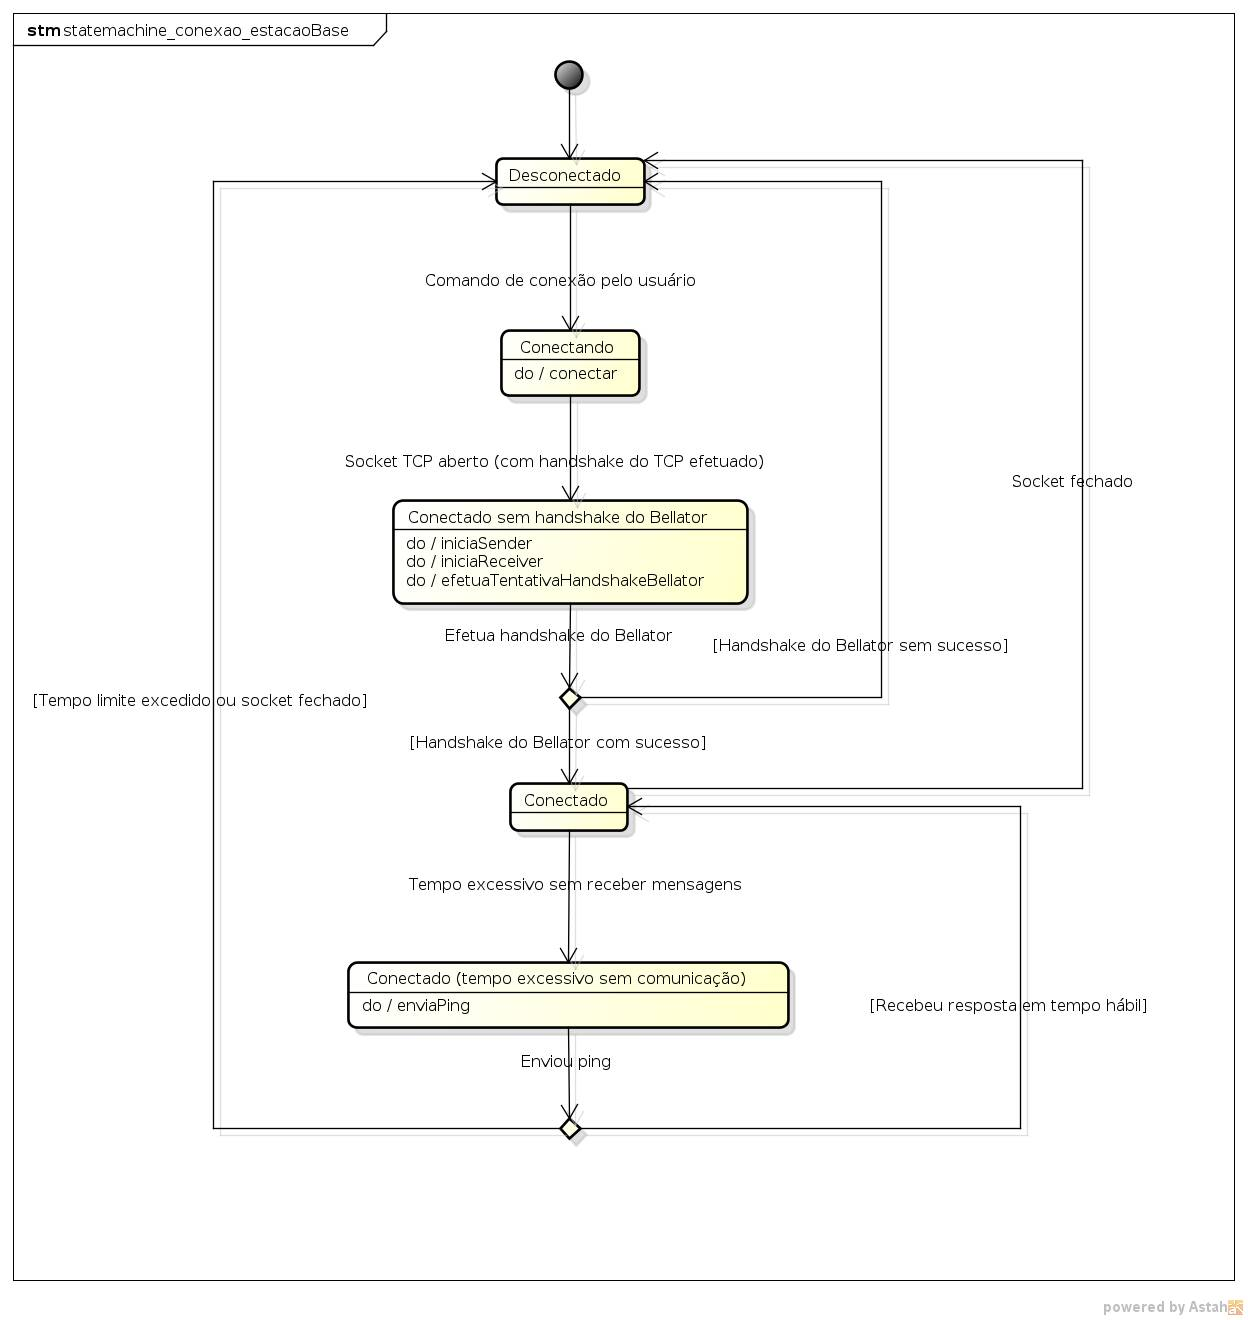
\includegraphics[width=\textwidth, keepaspectratio]{./figuras/estacaoBase/statemachine_conexao_estacaoBase.jpg}
  \caption{Diagrama estados da \textit{thread} principal da conexão da estação base.}
  \label{fig:diagrama_estados_estacao_base}
\end{figure}

\begin{figure}[H]
  \centering
  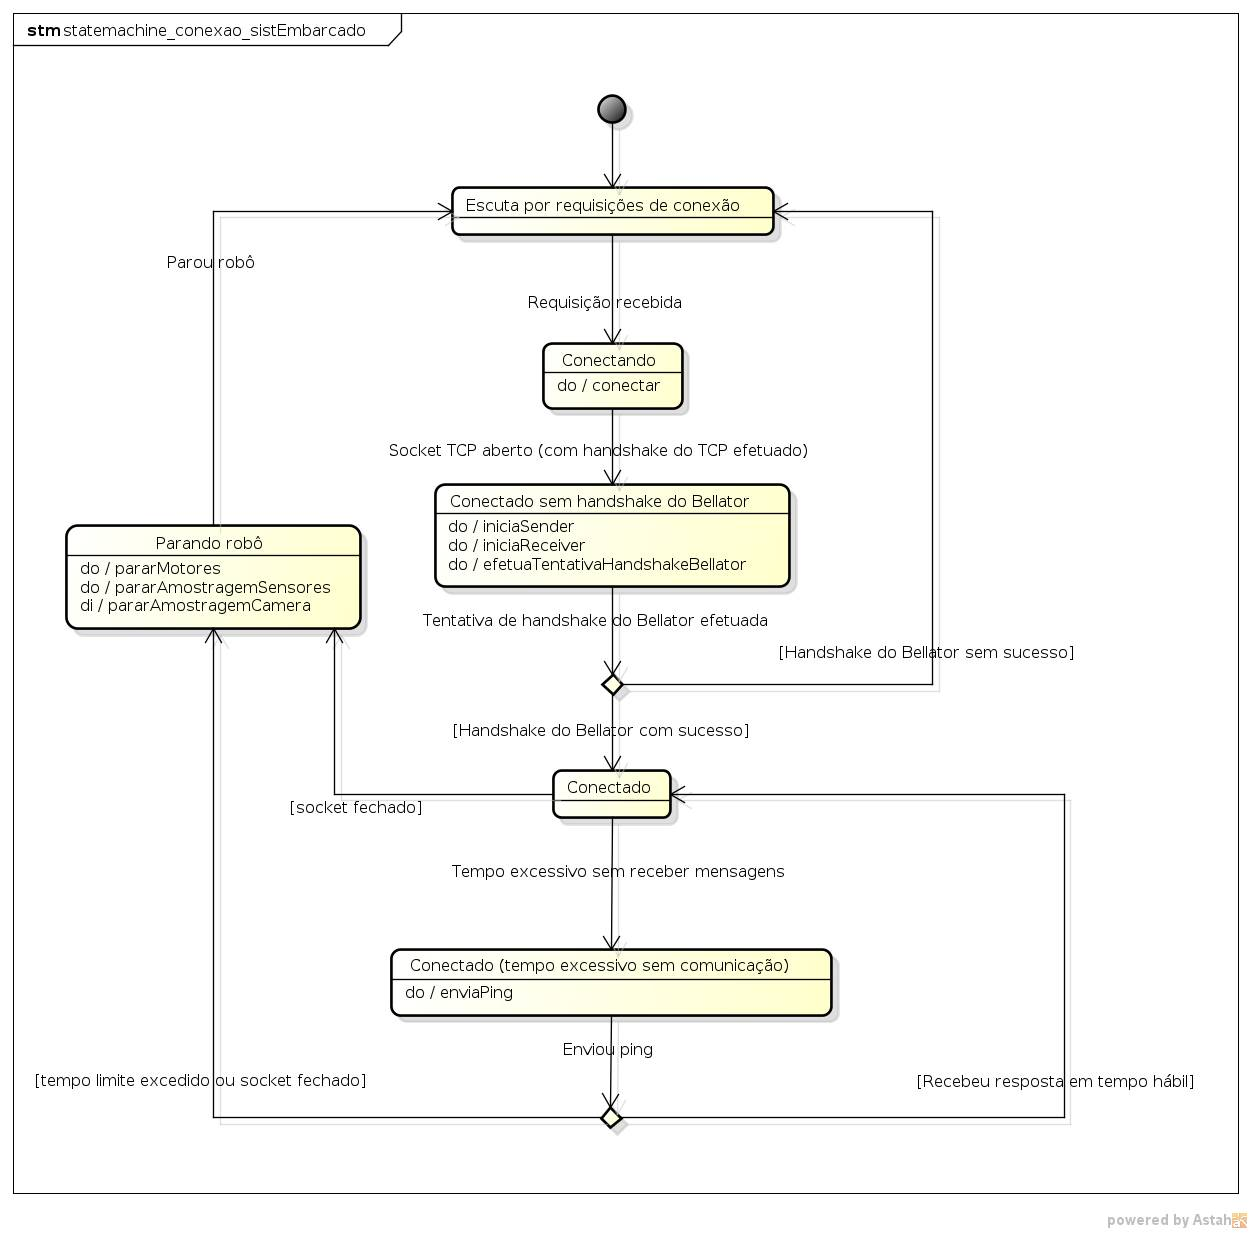
\includegraphics[width=\textwidth, keepaspectratio]{./figuras/sistEmbarcado/statemachine_conexao_sistEmbarcado.jpg}
  \caption{Diagrama de estados da \textit{thread} principal da conexão do linux embarcado.}
  \label{fig:diagrama_estados_sist_embarcado}
\end{figure}

\begin{figure}[H]
  \centering
  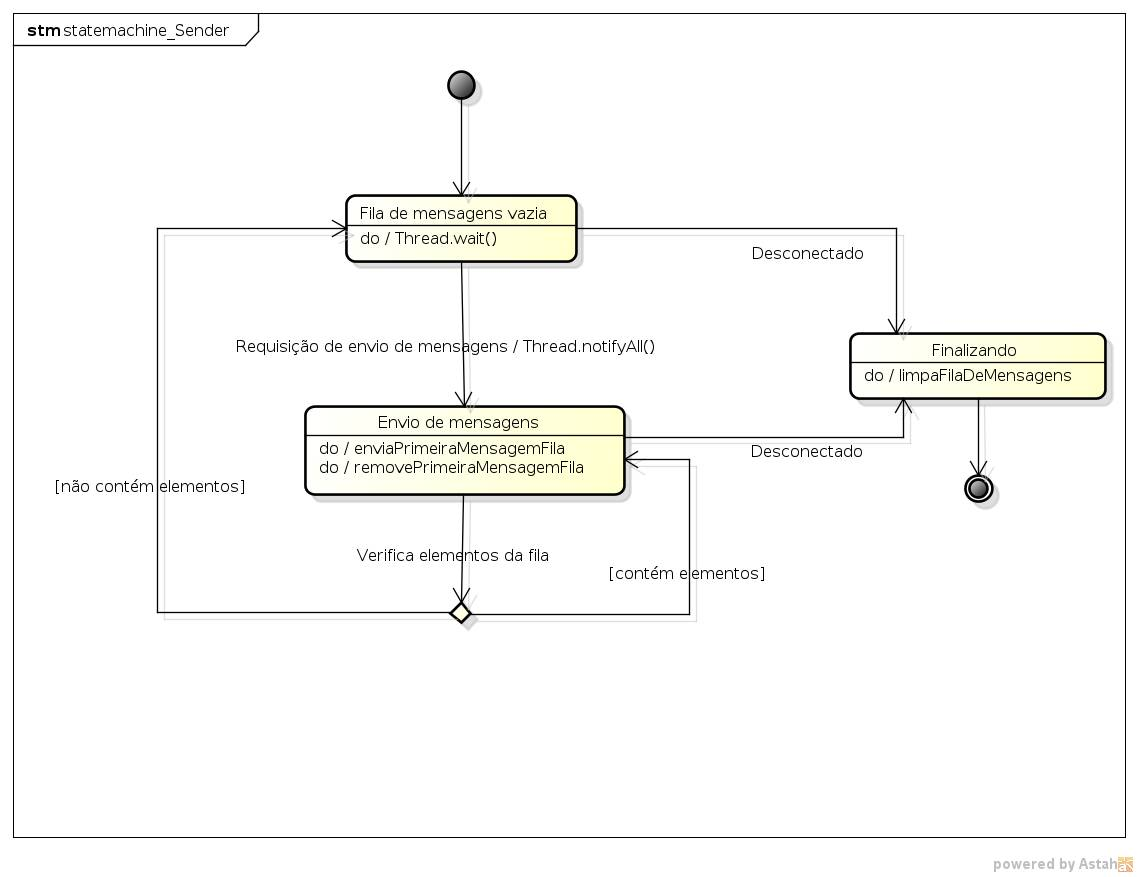
\includegraphics[width=\textwidth, keepaspectratio]{./figuras/statemachine_Sender.jpg}
  \caption{Diagrama de estados da \textit{thread} que envia mensagens (igual para estação base e linux embarcado).}
  \label{fig:diagrama_estados_sender}
\end{figure}

\begin{figure}[H]
  \centering
  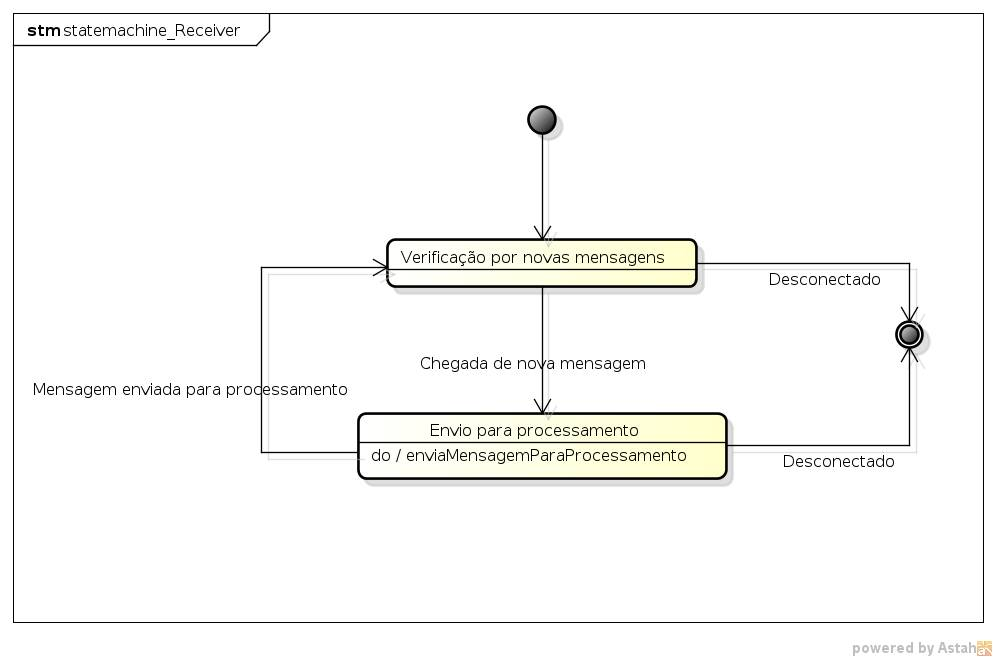
\includegraphics[width=\textwidth, keepaspectratio]{./figuras/statemachine_Receiver.jpg}
  \caption{Diagrama de estados da \textit{thread} receptora de mensagens (igual para estação base e linux embarcado).}
  \label{fig:diagrama_estados_receiver}
\end{figure}

\begin{figure}[H]
  \centering
  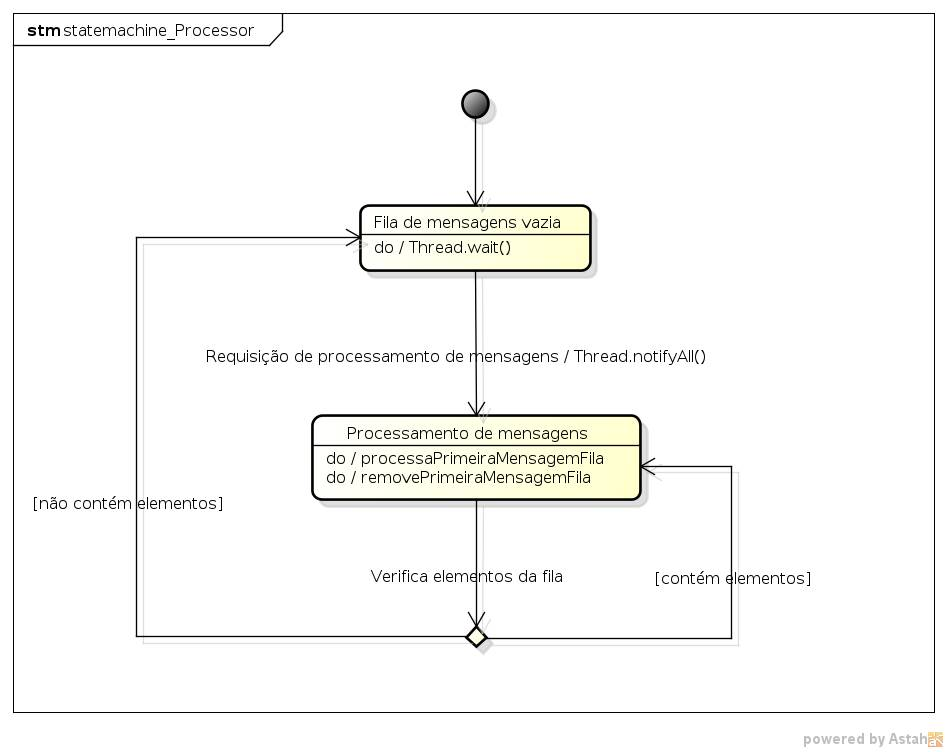
\includegraphics[width=\textwidth, keepaspectratio]{./figuras/statemachine_Processor.jpg}
  \caption{Diagrama de estados da \textit{thread} que processa mensagens recebidas (igual para estação base e linux embarcado).}
  \label{fig:diagrama_estados_processor}
\end{figure}

\begin{figure}[H]
  \centering
  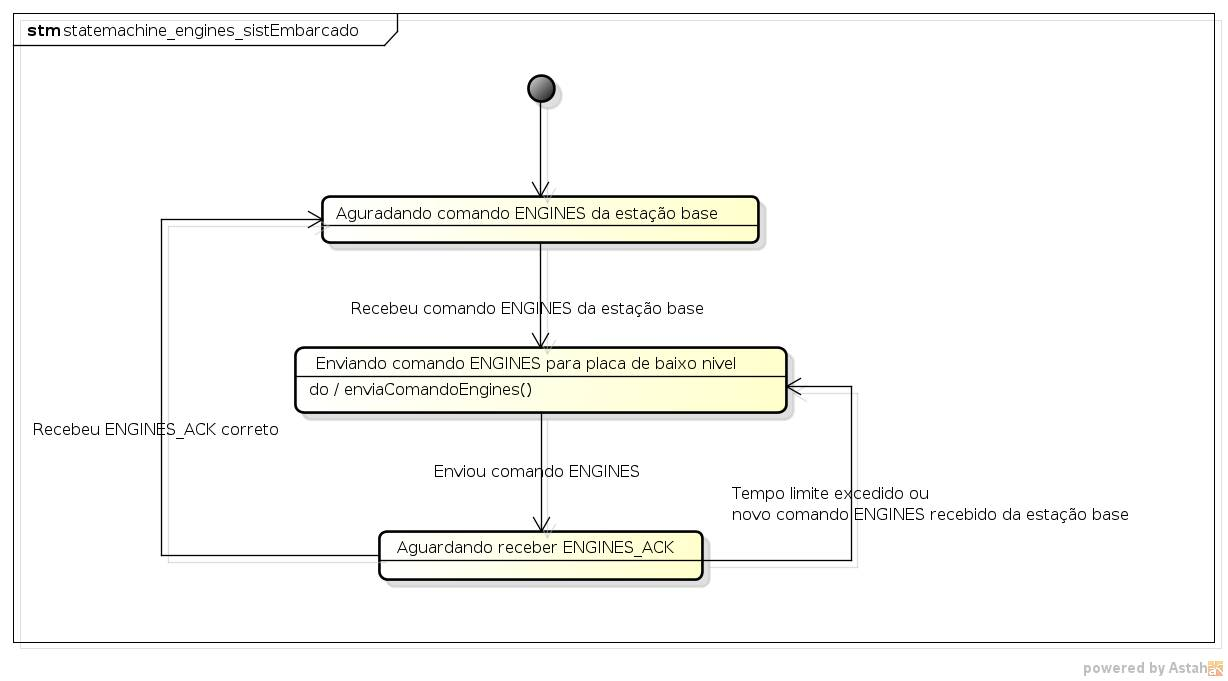
\includegraphics[width=\textwidth, keepaspectratio]{./figuras/sistEmbarcado/statemachine_motores_sistEmbarcado.jpg}
  \caption{Diagrama de estados da \textit{thread} responsável por gerenciar os comandos dos motores (linux embarcado).}
  \label{fig:diagrama_estados_motores_sist_embarcado}
\end{figure}

\begin{figure}[H]
  \centering
  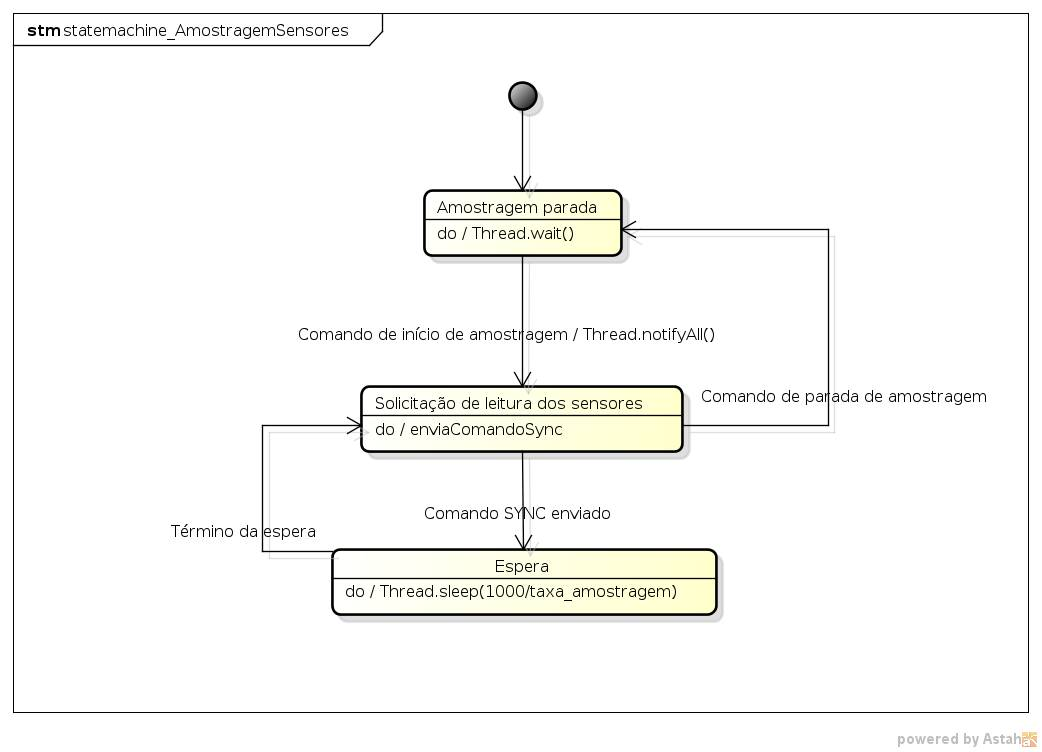
\includegraphics[width=\textwidth, keepaspectratio]{./figuras/sistEmbarcado/statemachine_AmostragemSensores_sistEmbarcado.jpg}
  \caption{Diagrama de estados da \textit{thread} responsável por efetuar a amostragem dos sensores (linux embarcado).}
  \label{fig:diagrama_estados_amostragem_sensores_sist_embarcado}
\end{figure}

\begin{figure}[H]
  \centering
  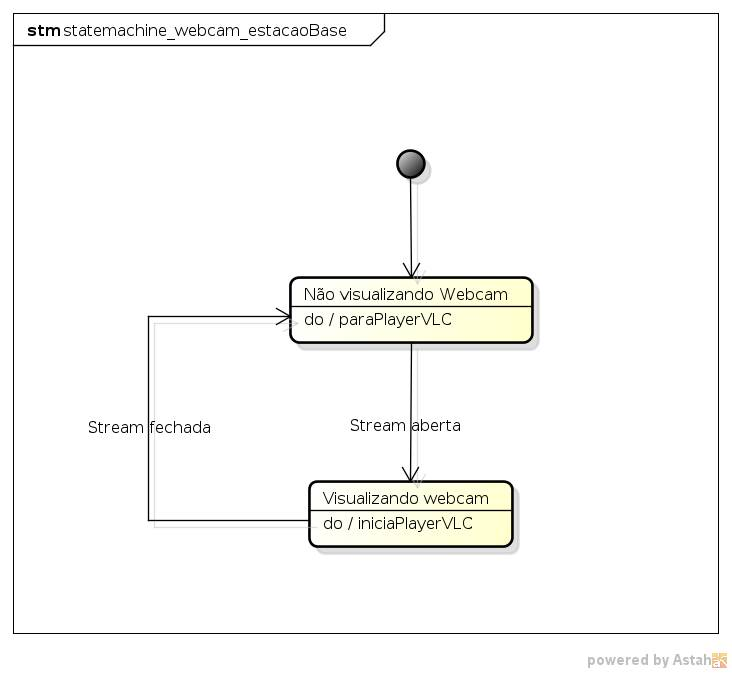
\includegraphics[width=\textwidth, keepaspectratio]{./figuras/estacaoBase/statemachine_webcam_estacaoBase.jpg}
  \caption{Diagrama de estados do visualização de imagens da \textit{webcam} (estação base).}
  \label{fig:diagrama_estados_webcam_estacao_base}
\end{figure}

\begin{figure}[H]
  \centering
  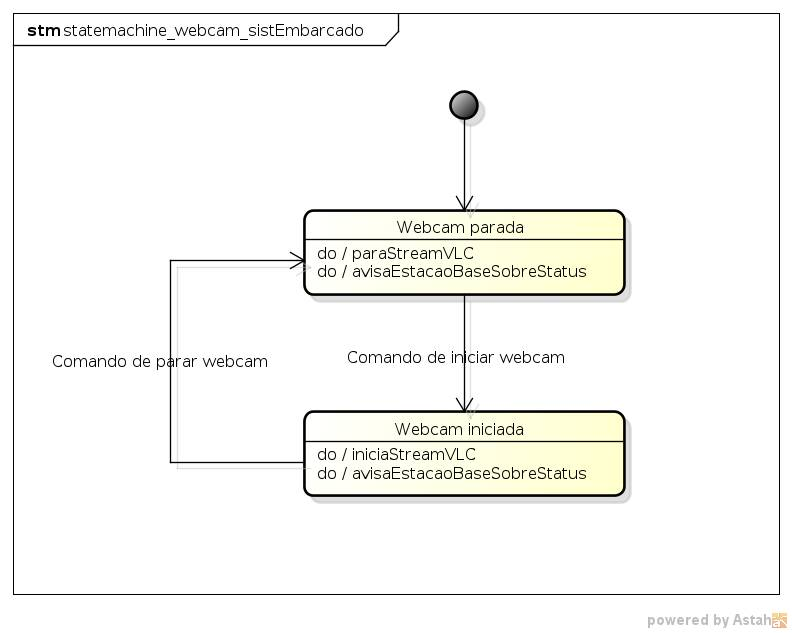
\includegraphics[width=\textwidth, keepaspectratio]{./figuras/sistEmbarcado/statemachine_webcam_sistEmbarcado.jpg}
  \caption{Diagrama de estados do envio de imagens da \textit{webcam} (linux embarcado).}
  \label{fig:diagrama_estados_webcam_sist_embarcado}
\end{figure}



\subsection{Diagramas de sequência}

Nessa seção os diagramas de sequência de comandos dos motores, de mensagens de amostras dos sensores e da ativação da webcam. Os diagramas das Figuras \ref{fig:diagrama_sequencia_motores_estacao_base} e \ref{fig:diagrama_sequencia_motores_sist_embarcado} representam como um comando de mudança de velocidade das rodas dado pelo usuário chega até a placa de baixo nível. Os das Figuras \ref{fig:diagrama_sequencia_sensores_sist_embarcado} e \ref{fig:diagrama_sequencia_sensores_estacao_base} demonstram a sequência dos dados de leituras dos sensores que saem da placa de baixo nível e chegam até o usuário.  Os diagramas das Figuras \ref{fig:diagrama_sequencia_webcam_estacao_base} e \ref{fig:diagrama_sequencia_webcam_sist_embarcado} demonstram um comando de ativação da webcam dado pelo usuário, como ele chega até o Linux embarcado e como posteriormente o usuário recebe as imagens da webcam.

Vale ressaltar que as chamadas assíncronas, ou seja, que não bloqueiam a execução da \textit{thread} chamadora, foram representadas também nestes diagramas.

\begin{figure}[H]
  \centering
  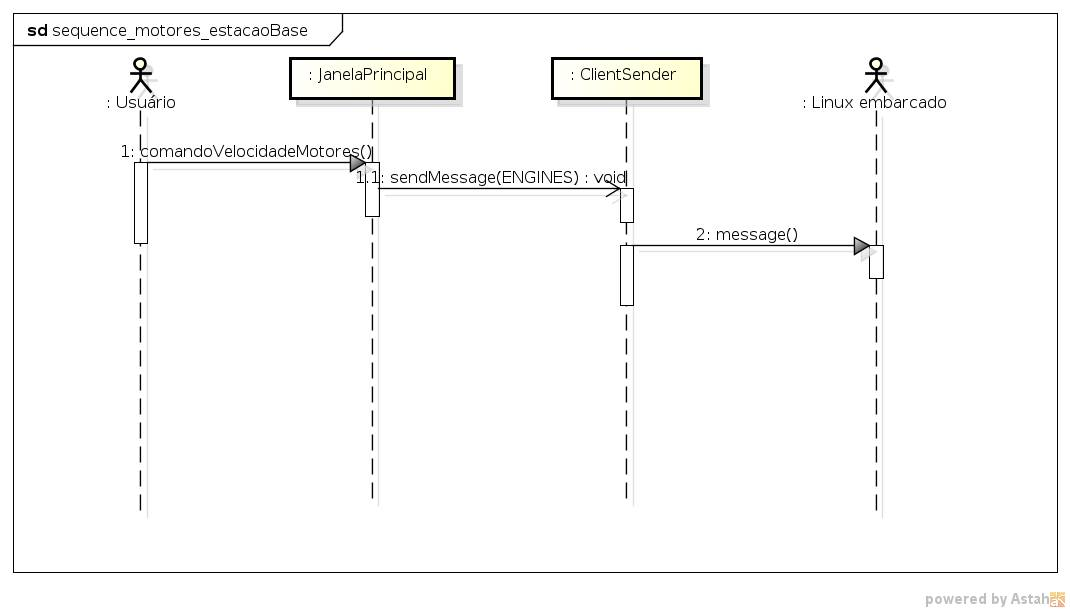
\includegraphics[width=\textwidth, keepaspectratio]{./figuras/estacaoBase/sequence_motores_estacaoBase.jpg}
  \caption{Diagrama de sequência de comando para mudança de velocidade dos motores (representa comando dado pelo usuário).}
  \label{fig:diagrama_sequencia_motores_estacao_base}
\end{figure}

\begin{figure}[H]
  \centering
  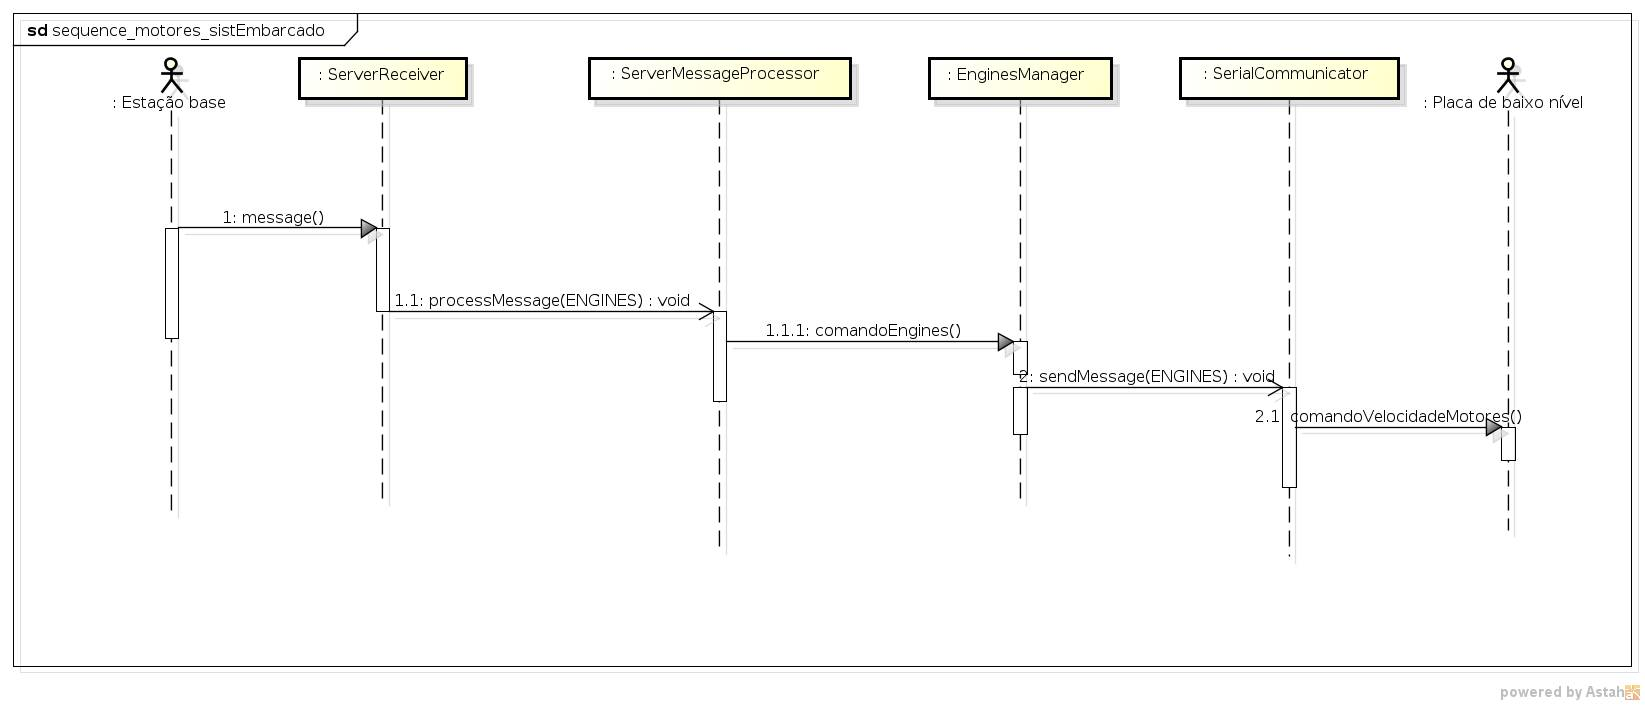
\includegraphics[width=\textwidth, keepaspectratio]{./figuras/sistEmbarcado/sequence_motores_sistEmbarcado.jpg}
  \caption{Diagrama de sequência de comando para mudança de velocidade dos motores (representa mensagem chegando no sistema embarcado).}
  \label{fig:diagrama_sequencia_motores_sist_embarcado}
\end{figure}

\begin{figure}[H]
  \centering
  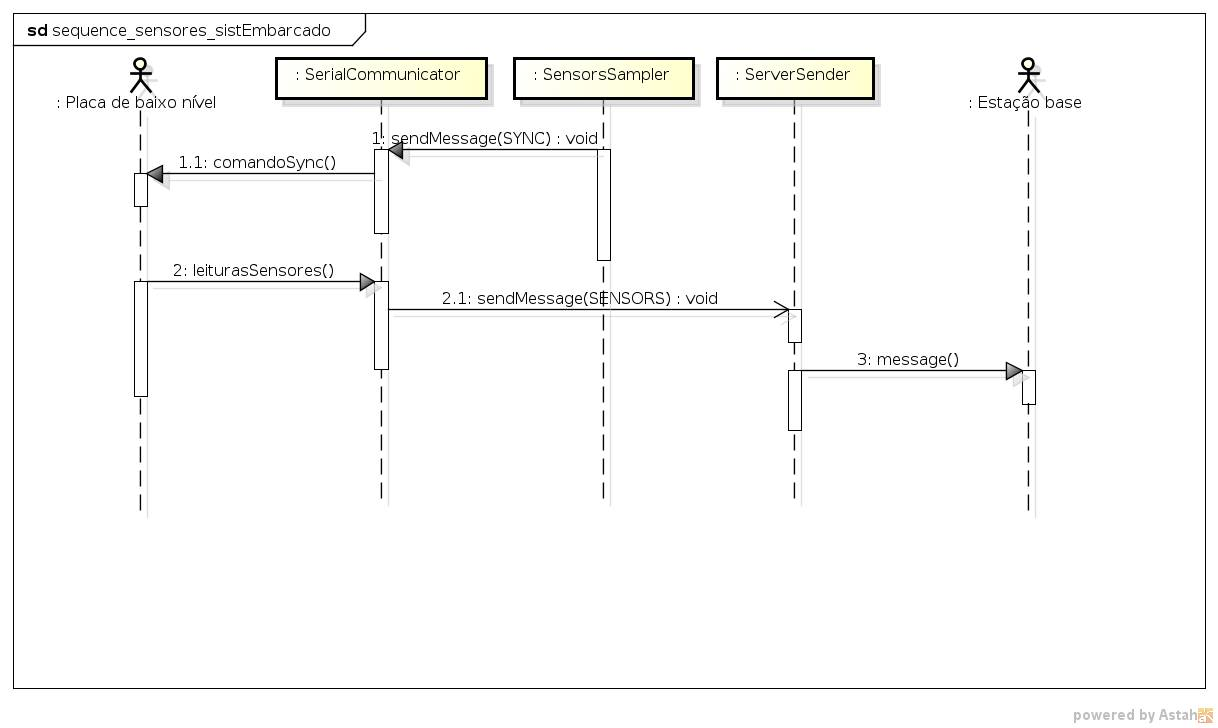
\includegraphics[width=\textwidth, keepaspectratio]{./figuras/sistEmbarcado/sequence_sensores_sistEmbarcado.jpg}
  \caption{Diagrama de sequência da amostragem dos sensores (representa amostras saindo do sistema embarcado).}
  \label{fig:diagrama_sequencia_sensores_sist_embarcado}
\end{figure}

\begin{figure}[H]
  \centering
  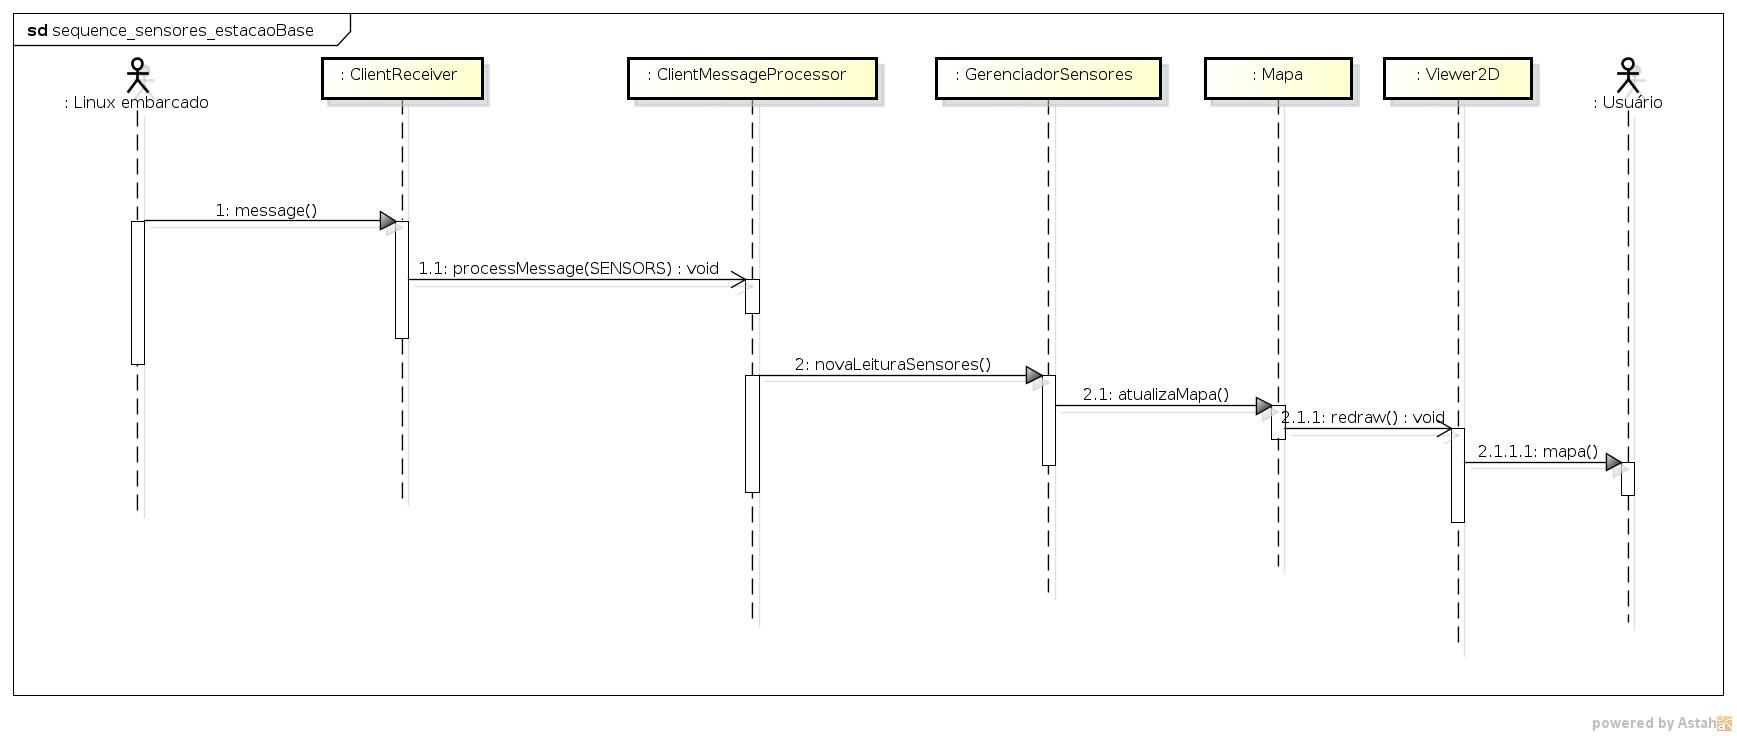
\includegraphics[width=\textwidth, keepaspectratio]{./figuras/estacaoBase/sequence_sensores_estacaoBase.jpg}
  \caption{Diagrama de sequência da amostragem dos sensores (representa mensagem chegando na estação base).}
  \label{fig:diagrama_sequencia_sensores_estacao_base}
\end{figure}

\begin{figure}[H]
  \centering
  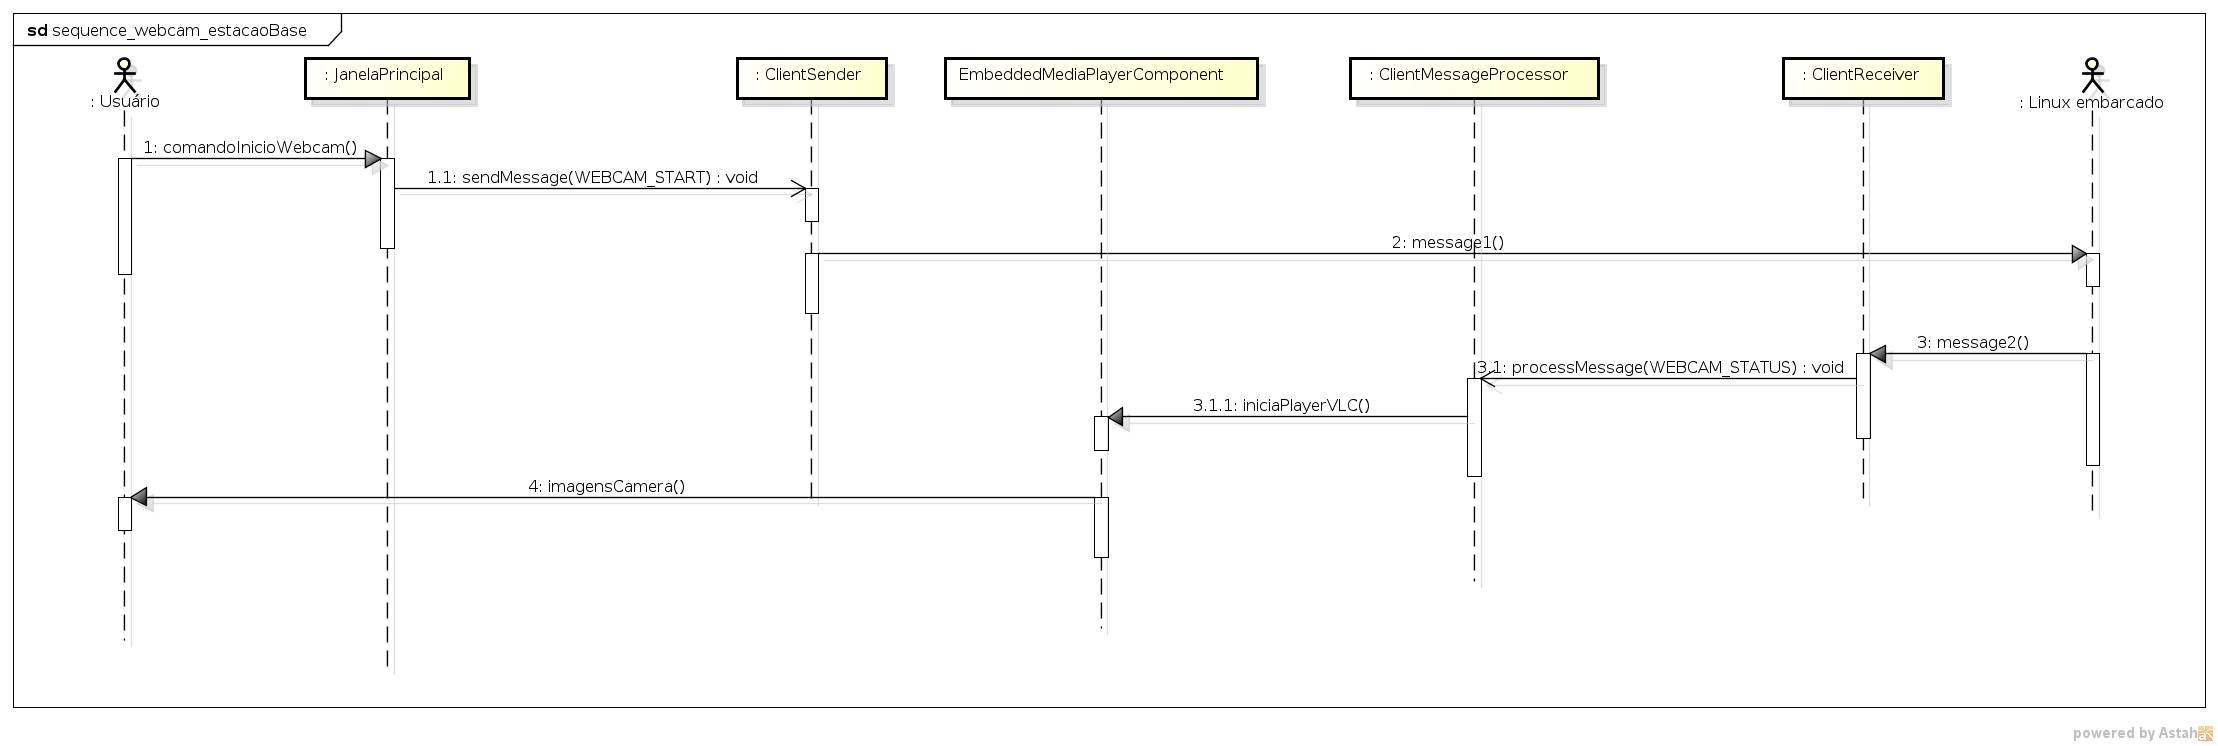
\includegraphics[width=\textwidth, keepaspectratio]{./figuras/estacaoBase/sequence_webcam_estacaoBase.jpg}
  \caption{Diagrama de sequência de comando para ativação da webcam (representa comando dado pelo usuário e o \textit{player} da \textit{libVLC} sendo ativado posteriormente).}
  \label{fig:diagrama_sequencia_webcam_estacao_base}
\end{figure}

\begin{figure}[H]
  \centering
  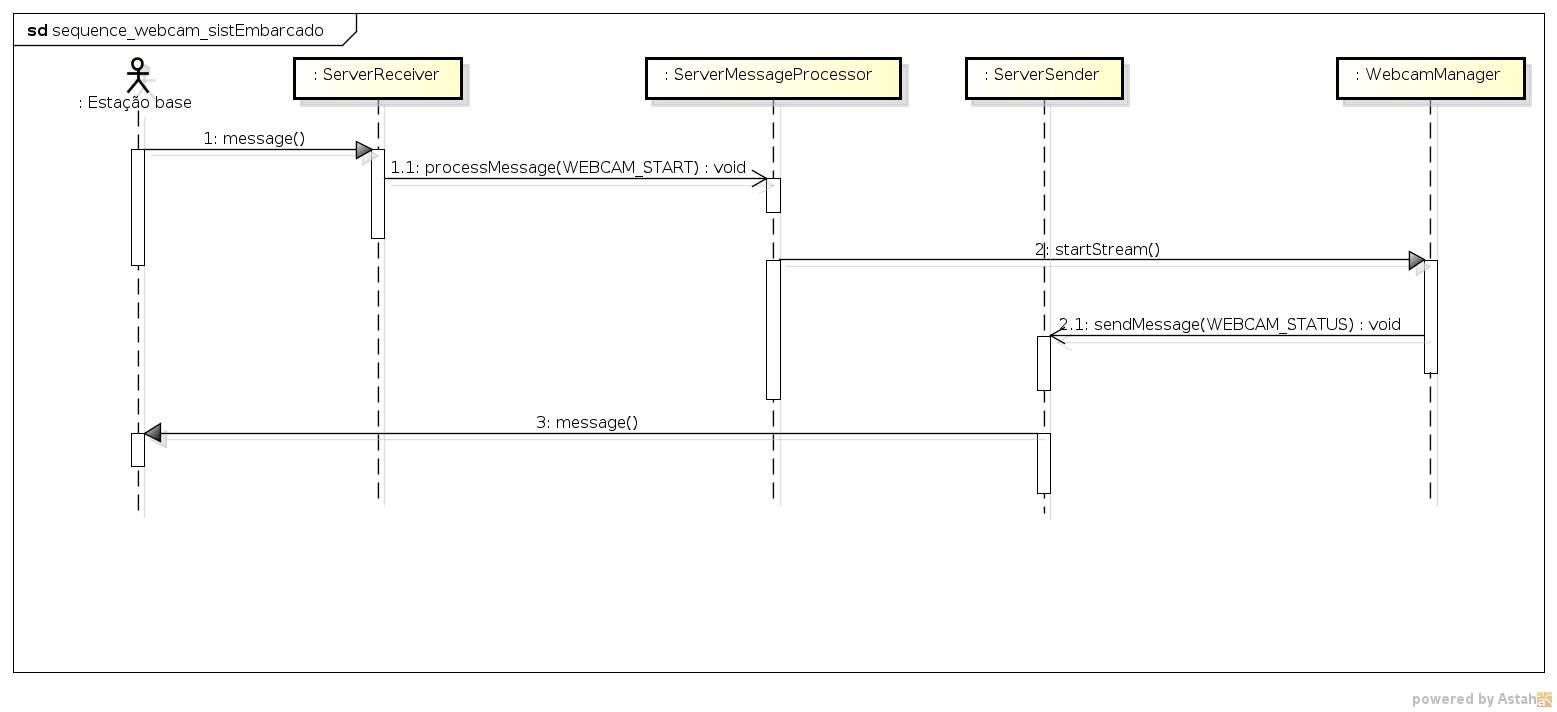
\includegraphics[width=\textwidth, keepaspectratio]{./figuras/sistEmbarcado/sequence_webcam_sistEmbarcado.jpg}
  \caption{Diagrama de sequência de comando para ativação da webcam (representa mensagem de ativação da webcam chegando no sistema embarcado e estação base sendo posteriormente notificada sobre o novo status).}
  \label{fig:diagrama_sequencia_webcam_sist_embarcado}
\end{figure}




\chapter{Diagrama de blocos do hardware}
Na figura \ref{fig:diagrama_blocos_hardware} mostra-se o diagrama de blocos do sistema embarcado e suas conexões com o restante do robô. A seguir está também uma descrição para cada um dos blocos da placa de circuito impresso do sistema embarcado.

\begin{figure}[H]
  \centering
  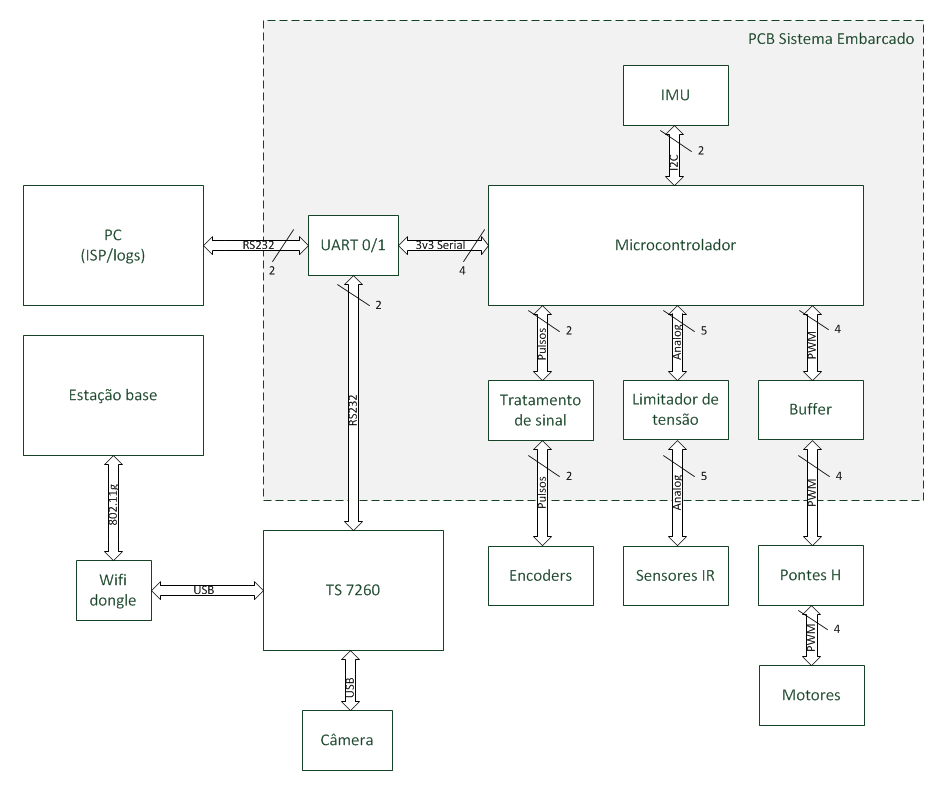
\includegraphics[width=\textwidth]{./figuras/diagrama_blocos_hardware.png}
  \caption{Diagrama de blocos do hardware}
  \label{fig:diagrama_blocos_hardware}
\end{figure}


\begin{enumerate}[topsep=0pt, partopsep=0pt, itemsep=0pt]
    \item Microcontrolador: Este bloco fará a leitura dos sensores: encoders, infra-vermelhos, acelerômetro e giroscópios. Além disso possui a implementação do protocolo de comunicação para interação com o linux embarcado da placa TS-7260.
    \item UART 0/1: Responsável por ajustar os níveis de tensão para comunicação serial no padrão RS-232 com a placa TS-7260.
    \item Buffer: Responsável por fornecer corrente e elevar os níveis de tensão de saída do microcontrolador de 3,3V para 5,0V. Esse buffer é conectado às pontes H já existentes no robô.
    \item IMU: possui o acelerômetro e o giroscópio e se comunicará com o microcontrolador por meio do protocolo I2C.
    \item Limitador de tensão: Necessário pois os sinais de saída dos sensores de infravermelho que já existem no robô não estão limitados em 5V, podendo a saída ultrapassar 5,0V e danificar o microcontrolador. 
    \item Tratamento de sinal: Composto por um filtro RC passa baixas e um schmitt trigger para remover qualquer falha que possa ocorrer na geração dos pulsos no encoder. A frequência de corte do filtro pode ser obtida pela velocidade máxima que o robô pode atingir, que foi suposta em 1 m/s (como apresentado nos requisitos de hardware).
\end{enumerate}



\chapter{Geração do mapa}

A posição do robô no mapa em cada instante é representada por um ponto no plano cartesiano e por um ângulo, que indica para qual sentido o robô está orientado. Esse ponto no plano indica onde está o centro de movimento do robô, que é o ponto médio entre as duas rodas.

Neste projeto, a determinação do deslocamento do robô é determinada primariamente pelos encoders presentes cada roda. O acelerômetro e o giroscópio são utilizados para aumentar a confiabilidade dos cálculos de deslocamento, principalmente em caso de escorregamento das rodas.

Na próxima seção será explicada a teoria da determinação do deslocamento, velocidade e aceleração do centro de movimento do robô a partir das leituras dos encoders em cada instante. Na seção \ref{sec:teoria_acel_giro} será explicitada a forma como as leituras do acelerômetro e giroscópio serão utilizadas para aumentar a confiabilidade das medições.

Na Figura \ref{fig:robo} está presente um esquema básico do robô visto de cima e virado com a frente para a direita. Nessa figura estão presentes os nomes das variáveis que são utilizadas nos cálculos posteriores.

\begin{figure}[H]
  \centering
  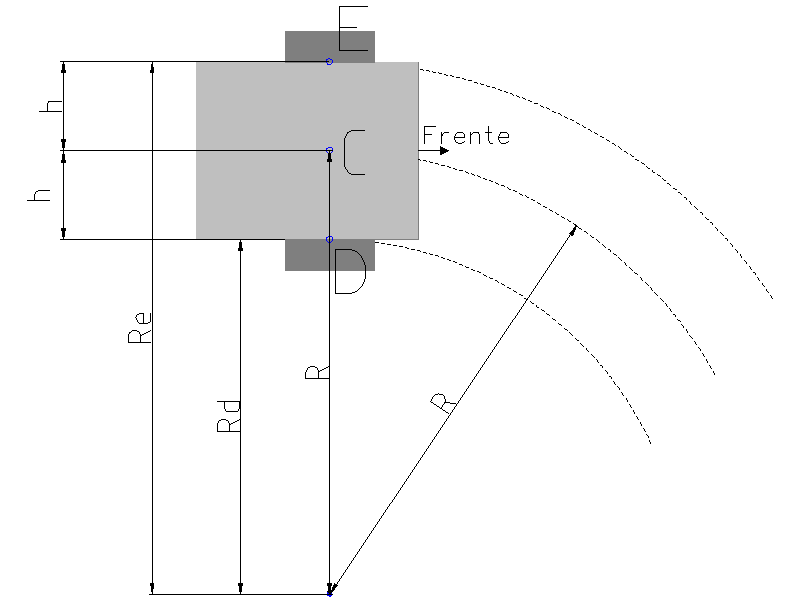
\includegraphics[width=0.5\textwidth, keepaspectratio]{./figuras/robo/robo.png}
  \caption{Representação básica do robô (visão superior).}
  \label{fig:robo}
\end{figure}

\section{Encoders}

Há dois dados importantes a determinar sobre o deslocamento do centro de movimento do robô: o deslocamento linear (distância absoluta percorrida) e o angular (variação do ângulo de orientação do robô). Cada encoder fornece uma medida de contagem de pulsos por volta a cada intervalo de amostragem. 

Na Figura \ref{fig:roda_encoder} está presente um representação básica de uma roda, acoplada a um encoder. Os números da figura são utilizados como índices nos cálculos explicitados posteriormente.

\begin{figure}[H]
  \centering
  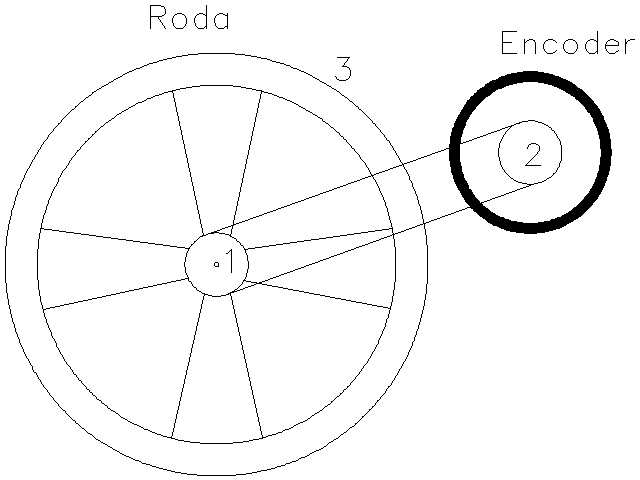
\includegraphics[width=0.5\textwidth, keepaspectratio]{./figuras/robo/roda_encoder.png}
  \caption{Representação de uma roda acoplada a um encoder.}
  \label{fig:roda_encoder}
\end{figure}

\subsection{Deslocamento de cada roda}

Um princípio importante utilizado nos cálculos é a relação entre o deslocamento $\Delta x$ ao redor de uma circunferência (de raio $R$) e a variação do ângulo $\Delta \theta$:

\begin{equation}
  \Delta x = R \cdot \Delta \theta
  \label{eq:deslocamento_circunferencia}
\end{equation}

Nos cálculos a seguir, faz-se uso do índice 1 para o eixo da roda, 2 para o eixo do encoder e 3 para a própria roda, de acordo com a figura \ref{fig:roda_encoder}. Para determinar a distância percorrida pela roda, deve-se considerar a circunferência do eixo da roda ($C_1$), a circunferência do eixo do encoder ($C_2$) e a circunferência da roda ($C_3$).

O acoplamento do eixo do encoder com o eixo da roda é feita por uma correia de borracha, e portanto considera-se que o deslocamento ($ \Delta x_1$) na superfície do eixo da roda é igual ao deslocamento ($ \Delta x_2$) na superfície do eixo do encoder. Pode-se, com isso, calcular:

\begin{eqnarray*}
   \Delta x_1 =  \Delta x_2 \rightarrow \Delta \theta_1 R_1 = \Delta \theta_2 R_2 \rightarrow \Delta \theta_1 \frac{C_1}{2 \pi} = \Delta \theta_2 \frac{C_2}{2 \pi} 
\end{eqnarray*}

\begin{equation}
  \Delta \theta_1 = \frac{C_2}{C_1} \cdot \Delta \theta_2
  \label{eq:theta1_theta2}
\end{equation}

Calculando-se a relação entre a contagem de pulsos do encoder ($E$) e o ângulo de rotação ($\Delta \theta_2$) do eixo do encoder, levando-se em conta que há uma contagem de 1800 pulsos por volta:

\begin{equation}
  \Delta \theta_2 = \frac{2 \pi}{1800} \cdot E \unit{rad}
  \label{eq:E_theta2}
\end{equation}

Substituindo-se a equação \ref{eq:E_theta2} na \ref{eq:theta1_theta2}, tem-se que:

\begin{equation}
  \Delta \theta_1 = \frac{C_2}{C_1} \frac{2 \pi}{1800} \cdot E \unit{rad}
  \label{eq:theta_1}
\end{equation}

Calculando-se a relação entre a variação do ângulo do eixo da roda ($\Delta \theta_1$) e o deslocamento da roda ($x_3$):

\begin{eqnarray*}
  \Delta \theta_1 = \Delta \theta_3 \rightarrow \Delta \theta_1 =  \Delta x_3 R_3 \rightarrow \Delta \theta_1 = \Delta x_3 \frac{C_3}{2 \pi} \rightarrow  \Delta x_3 = \Delta \theta_1 \frac{2 \pi}{C_3}
\end{eqnarray*}

Substituindo-se o valor de ($\Delta \theta_1$) da equação \ref{eq:theta_1}:

\begin{eqnarray*}
   \Delta x_3 = \frac{C_2}{C_1} \frac{2 \pi}{1800} \cdot E \cdot \frac{2 \pi}{C_3} = \frac{C_2}{C_1 C_3} \frac{(2 \pi)^2}{1800} \cdot E
\end{eqnarray*}

\begin{empheq}[box=\fbox]{equation}
   \Delta x_3 = \frac{C_2}{C_1 C_3} \frac{\pi^2}{450} \cdot E
  \label{eq:x_3}
\end{empheq}


Que é o valor do deslocamento da roda em função da contagem de pulsos do encoder. 


\subsection{Deslocamento do centro de movimento do robô}

Como já explicitado anteriormente, o centro de movimento do robô considerado é o ponto médio entre as duas rodas. As duas variáveis para determinar em cada instante de tempo são o deslocamento linear (distância absoluta percorrida) e o angular (variação do ângulo de orientação do robô). Considerando-se que em cada instante o robô descreve um movimento circular uniforme (MCU), o raio da trajerória deve ser determinado para que os cálculos de posicionamento do robô possam ser feitos. Este raio depende do deslocamento das rodas em cada instante, e é uma importante variável que será estudada na próxima subseção.

Nos cálculos que serão explicitados a seguir, utiliza-se o índice E para a roda esquerda, C para o centro de movimento do robô e D para a roda direita.

Uma relação importante a notar a princípio é que a variação do ângulo de orientação em cada instante é igual nos três pontos: E (roda esquerda), C (centro de movimento) e D (roda direita), visto que todos estão fixos em relação à carcaça do robô. Parte-se da seguinte relação fundamental, portanto:

\begin{equation}
  \Delta \theta_E = \Delta \theta_D = \Delta \theta_C
  \label{eq:relacao_fundamental_theta}
\end{equation}



\subsubsection{Raio do movimento}

Para determinar o raio ($R$) descrito pelo centro de movimento do robô em sua trajetória instantânea em MCU, usa-se os dois primeiros termos da igualdade da equação \ref{eq:relacao_fundamental_theta}:

\begin{eqnarray*}
  \Delta \theta_E = \Delta \theta_D \rightarrow \frac{\Delta x_E}{R_E} = \frac{\Delta x_D}{R_D} 
\end{eqnarray*}

Mas:
\begin{equation*}
  R_E = R + h, ~ ~ R_D = R - h
\end{equation*}

Portanto:

\begin{eqnarray*}
  \frac{\Delta x_E}{R + h} = \frac{\Delta x_D}{R - h} ~\rightarrow~ \frac{\Delta x_E}{\Delta x_D} = \frac{R + h}{R - h} ~\rightarrow~ \frac{\Delta x_E (R - h)}{\Delta x_D} = R + h 
\end{eqnarray*}
\begin{eqnarray*}
  \frac{\Delta x_E \cdot R - \Delta x_E \cdot h}{\Delta x_D} = R + h ~\rightarrow~ 
  \frac{\Delta x_E}{\Delta x_D} \cdot R - \frac{\Delta x_E}{\Delta x_D} \cdot h = R + h ~\rightarrow~ 
  \frac{\Delta x_E}{\Delta x_D} \cdot R - R = \frac{\Delta x_E}{\Delta x_D} \cdot h + h
\end{eqnarray*}
\begin{eqnarray*}
  R \left( \frac{\Delta x_E}{\Delta x_D} - 1 \right) = h \left( \frac{\Delta x_E}{\Delta x_D} + 1 \right) ~\rightarrow~
  R = h \cdot \frac{\left( \frac{\Delta x_E}{\Delta x_D} + 1 \right)}{\left( \frac{\Delta x_E}{\Delta x_D} - 1 \right)}  ~\rightarrow~
  R = h \cdot \frac{\frac{\Delta x_E + \Delta x_D}{x_D}}{\frac{\Delta x_E - \Delta x_D}{\Delta x_D}} 
\end{eqnarray*}

\begin{empheq}[box=\fbox]{equation}
  R = h \cdot \frac{\Delta x_E + \Delta x_D} {\Delta x_E - \Delta x_D}
  \label{eq:R}
\end{empheq}

Vê-se que o raio $R$ do movimento circular uniforme em cada instante depende do deslocamento de cada roda ($\Delta x_E$ e $\Delta x_D$) e da distãncia $h$ entre as rodas e o centro de movimento do robô.


\subsubsection{Deslocamento linear} 

Para calcular o deslocamento linear do centro de movimento do robô, usa-se os dois últimos termos da equação \ref{eq:relacao_fundamental_theta}. Vale ressaltar que poderiam ser escolhidos também o primeiro e o último termos, pois o resultado obtido seria idêntico. Tem-se que:

\begin{eqnarray*}
  \Delta \theta_D = \Delta \theta_C \rightarrow \frac{\Delta x_D}{R_D} = \frac{\Delta x_C}{R} 
\end{eqnarray*}

Mas:
\begin{equation*}
  R_D = R - h
\end{equation*}

Portanto:
\begin{eqnarray*}
  \frac{\Delta x_D}{R - h} = \frac{\Delta x_C}{R} ~\rightarrow~ x_D = x_C \cdot \frac{R - h}{R} 
\end{eqnarray*}

Substituindo-se o valor de $R$ da equação \ref{eq:R}:
\begin{eqnarray*}
  \Delta x_D = \Delta x_C \left[ \frac{h \cdot \frac{\Delta x_E + \Delta x_D}{\Delta x_E - \Delta x_D} - h}{h \cdot \frac{\Delta x_E + \Delta x_D}{\Delta x_E - \Delta x_D}} \right]
\end{eqnarray*}

Dividindo-se o numerador e denominador do segundo termo por $h$:
\begin{equation*}
  \Delta x_D = \Delta x_C \left[ \frac{\frac{\Delta x_E + \Delta x_D}{\Delta x_E - \Delta x_D} - 1}{\frac{\Delta x_E + \Delta x_D}{\Delta x_E - \Delta x_D}} \right]
\end{equation*}

Multiplicando-se o numerador e denominador do segundo termo por $\frac{\Delta x_E - \Delta x_D}{\Delta x_E + \Delta x_D}$:

\begin{equation*}
  \Delta x_D = \Delta x_C \left[1 - \frac{\Delta x_E - \Delta x_D}{\Delta x_E + \Delta x_D} \right] ~\rightarrow~
  \Delta x_D = \Delta x_C \left[\frac{(\Delta x_E + \Delta x_D) - (\Delta x_E - \Delta x_D)}{\Delta x_E + \Delta x_D} \right] 
\end{equation*}
\begin{equation*}
  \Delta x_D = \Delta x_C \cdot \left[ \frac{2 \Delta x_D}{\Delta x_E + \Delta x_D} \right] ~\rightarrow~
  \Delta x_C = \frac{\Delta x_D}{\left(\frac{2 \Delta x_D}{\Delta x_E + \Delta x_D} \right)}
\end{equation*}

\begin{empheq}[box=\fbox]{equation}
  \Delta x_C = \frac{\Delta x_E + \Delta x_D}{2}
  \label{eq:desloc_linear}
\end{empheq}

Notas-se que o deslocamento linear do centro de movimento do robô ($\Delta x_C$) é uma média simples dos dois deslocamentos lineares das rodas. Vê-se que ele não depende do raio de deslocamento nem da distância entre as duas rodas.


\subsubsection{Deslocamento angular}

O deslocamento angular ($\Delta \theta_c$) do centro de movimento do robô em cada instante pode ser calculado a partir do deslocamento linear e do raio do movimento circular uniforme. Usando-se a relação da equação \ref{eq:deslocamento_circunferencia}, tem-se que:


\begin{empheq}[box=\fbox]{equation}
  \Delta \theta_c = \frac{\Delta x_C}{R}
  \label{eq:desloc_angular}
\end{empheq}


Onde $\Delta x_C$ é o deslocamento linear do robô (equação \ref{eq:desloc_linear}) e $R$ é o raio do movimento circular uniforme (equação \ref{eq:R}). 

\subsubsection{Casos especiais}

Há dois casos especiais que devem ser considerados no cálculo do deslocamento (a partir dos dados dos encoders) do centro de movimento do robo. O primeiro é quando as duas rodas têm deslocamento igual ($\Delta x_E = \Delta x_D$). O raio do movimento circular (equação \ref{eq:R}) neste caso é:

\begin{equation}
  R = h \cdot \frac{\Delta x_E + \Delta x_D} {\Delta x_E - \Delta x_D} = h \cdot \frac{2 \cdot \Delta x_E}{0} \rightarrow \infty
  \label{eq:caso_especial1_R}
\end{equation}


O raio tende a infinito, o que implica que o deslocamento angular (equação \ref{eq:desloc_angular}) seja:

\begin{equation}
  \Delta \theta_c = \frac{\Delta x_C}{R} = \frac{\Delta x_C}{\infty} \rightarrow 0
  \label{eq:caso_especial1_theta}
\end{equation}

Já o deslocamento linear (equação \ref{eq:desloc_linear}) é:

\begin{equation}
  \Delta x_C = \frac{\Delta x_E + \Delta x_D}{2} = \frac{2 \Delta x_E}{2} = \Delta x_E
  \label{eq:caso_especial1_x}
\end{equation}

Isso corresponde à realidade, uma vez que quando as rodas têm deslocamentos iguais o robô está se deslocando sem fazer curvas. Não há deslocamento angular, portanto, e o deslocamento linear do centro de movimento é igual ao deslocamento de cada roda.

O segundo caso especial ocorre quando os deslocamento têm módulos iguais, porêm sentidos contrários (ou seja, $\Delta x_E = - \Delta x_D$). O raio nesse caso é:

\begin{equation}
  R = h \cdot \frac{\Delta x_E + \Delta x_D} {\Delta x_E - \Delta x_D} = h \cdot \frac{\Delta x_E - \Delta x_E}{\Delta x_E + \Delta x_E} = 0
    \label{eq:caso_especial2_R}
\end{equation}


O deslocamento linear (equação \ref{eq:desloc_linear}) é:

\begin{equation}
  \Delta x_C = \frac{\Delta x_E + \Delta x_D}{2} = \frac{\Delta x_E - \Delta x_E}{2} = 0
  \label{eq:caso_especial2_x}
\end{equation}

Esse valor corresponde à realidade, pois quando as rodas se deslocam em sentidos contários, e na mesma quantidade, o centro de movimento do robô não se desloca linearmente, mas apenas muda seu ângulo.
Usando-se a equação \ref{eq:desloc_angular}, tenta-se calcular o valor do deslocamento angular:

\begin{equation}
  \Delta \theta_c = \frac{\Delta x_C}{R} = \frac{0}{0}
  \label{eq:caso_especial2_theta}
\end{equation}

O valor obtido é indeterminado quando usa-se essa equação. Porém, analisando-se a natureza deste caso especial, pode ser notado que há um movimento circular cujo centro é o ponto médio entre as rodas (que é o centro de movimento do robô). O raio do MCU é a distância $h$ entre uma roda e o centro do robô, e o deslocamento ao longo da circunferência é o deslocamento de qualquer uma uma das rodas. Portanto, a equação \ref{eq:deslocamento_circunferencia} pode ser utilizada, isolando-se a variável $\theta$, para determinar o deslocamento angular do robô:

\begin{equation}
  \Delta \theta_c = \frac{\Delta x_E}{h}
  \label{eq:caso_especial2_theta2}
\end{equation}


\subsubsection{Velocidade e aceleraçao}

A velocidade e aceleração lineares do centro de movimento do robô podem ser calculadas por derivação numérica do deslocamento e velocidade em cada intervalo de tempo, considerando-se a velocidade e aceleração anteriores. Em cada intervalo discreto $n$:

\begin{equation}
  v_{c (n)} = \frac{x_{c (n)} - x_{c (n-1)}}{t_{(n)} - t_{(n-1)}}
  \label{eq:velocidade}
\end{equation}

\begin{equation}
  a_{c (n)} = \frac{v_{c (n)} - v_{c (n-1)}}{t_{(n)} - t_{(n-1)}}
  \label{eq:velocidade}
\end{equation}


A velocidade e aceleração angulares podem ser também obtidas por derivação numérica, considerando-se que o raio do movimento circular uniforme do robô é constante dentro do intervalo considerado. Em cada intervalo discreto $n$:

\begin{equation}
  \omega_{c (n)} = \frac{\theta_{c (n)} - \theta_{c (n-1)}}{t_{(n)} - t_{(n-1)}}
  \label{eq:velocidade}
\end{equation}

\begin{equation}
  \alpha_{c (n)} = \frac{\omega_{c (n)} - \omega_{c (n-1)}}{t_{(n)} - t_{(n-1)}}
  \label{eq:velocidade}
\end{equation}


\section{Acelerômetro e giroscópio}
\label{sec:teoria_acel_giro}

O acelerômetro e o giroscópio são utilizados para aumentar a confiabilidade dos dados de deslocamento do robô em caso de escorregamento das rodas.



Como definido na seção \ref{sec:codificacao_mensagens}, é recebido um valor de 2 bytes para cada eixo do acelerômetro. A faixa de funcionamento do acelerômetro está configurada em $-+2g$, logo a sensibilidade pelo \textit{datasheet} é de $16384 LSB/g$. Portanto, o valor de aceleração pode ser obtido pela fórmula:

\begin{equation}
  a = \frac{valorMedido}{16384} \cdot g \unit{m/s^2}
  \label{eq:acel}
\end{equation}

Onde g é a aceleração da gravidade ($9,80665 \unit{m/s^2}$). 

Para cada eixo do giroscópio, também e obtido um valor de 2 bytes. A faixa de funcionamento do giroscópio está configurada em $-+250$ graus/s, logo a sensibilidade pelo \textit{datasheet} é de 131 LSB/(graus/s). Portanto, o valor de velocidade angular pode ser obtida pela fórmula:

\begin{equation}
  \omega = \frac{valorMedido}{131} \unit{graus/s} = \frac{\pi}{180} \cdot \frac{valorMedido}{131} \unit{rad/s}
  \label{eq:giro}
\end{equation}


A princípio, apenas o eixo X do acelerômetro (voltado para a frente do robô) e o eixo Z do giroscópio (posicionado no sentido baixo/cima) serão utilizados para mapeamento, visto que poderão ser comparados facilmente com os dados obtidos pelos encoders. A ideia é posicioná-los no centro de movimento do robô (ponto médio entre as rodas) para que a comparação seja feita.

A velocidade e deslocamento lineares podem ser obtidos por integração numérica da aceleração linear em cada intervalo discreto $n$:

\begin{equation}
  v_{(n)} = v_{(n - 1)} + a_{(n)} \cdot (t_{(n)} - t_{(n-1)})
  \label{eq:v_acel}
\end{equation}

\begin{equation}
  \Delta x_{(n)} = \Delta x_{(n - 1)} + v_{(n)} \cdot (t_{(n)} - t_{(n-1)})
  \label{eq:v_acel}
\end{equation}

O deslocamento angular pode ser obtido por integração numérica da velocidade angular em cada intervalo discreto $n$:

\begin{equation}
  \Delta \theta_{(n)} = \Delta \theta_{(n - 1)} + \omega_{(n)} \cdot (t_{(n)} - t_{(n-1)})
  \label{eq:v_acel}
\end{equation}



\section{Sensores infra-vermelhos}

Para obter a posição em que cada obstáculo detectado está no mapa, primeiramente deve-se obter a distância detectada por cada sensor infra-vermelho. Como explicitado em \cite{bellator_2012}, o valor recebido em 1 byte do sensor pode ser convertido para a distãncia em centímetros pela fórmula (obtida por interpolação polinomial):

\begin{equation}
  y = 3,6404 \cdot 10^{-7} x^3 - 2,4435 \cdot 10^{-4} x^3 + 6,0732 \cdot 10^{-2} x^2 - 6,8962 x + 339,361
  \label{eq:IR_dist}
\end{equation}


Sendo $\overrightarrow{P_C}$ o vetor que sai da origem e vai até o centro de movimento do robô, $\overrightarrow{P_1}$ o vetor que vai do centro do robô até o sensor, e $\overrightarrow{P_2}$ o vetor que vai do sensor até o ponto do obstáculo detectado, faz-se a seguinte soma vetorial para encontrar o vetor $\overrightarrow{P}$, que é o ponto do obstáculo detectado no mapa:

\begin{equation}
  \overrightarrow{P} = \overrightarrow{P_C} + \overrightarrow{P_1} + \overrightarrow{P_2}
  \label{eq:IR_vector}
\end{equation}


O vetor $\overrightarrow{P_C}$ é determinado facilmente, pois é a última posição do robô. $\overrightarrow{P_1}$ é o vetor da posição do sensor relativa ao centro (informação obtida das configurações iniciais do robô), rotacionado pelo ângulo em que o robô está na última posição. $\overrightarrow{P_2}$ pode ser obtido criando-se um vetor com magnitude igual à distância detectada pelo sensor, e ângulo igual a: ângulo relativo do sensor no robô (informação obtida das configurações iniciais) somado com o ângulo em que o robô está na última posição.

\section{Algoritmo de posicionamento}

O algoritmo proposto para utilização dos vários sensores (encoder, acelerômetro e giroscópio) está exposto abaixo. Para cada amostra dos sensores recebida, o algoritmo efetua os seguintes passos:

\begin{enumerate}
      \item A partir das leituras dos encoders, calcular deslocamento linear ($x_e$, em metros) e angular ($\theta$, em $rad$) do centro de movimento do robô.
      \item Derivar duas vezes o deslocamento linear $x_e$ para obter aceleração linear ($a_e$, em $m/s^2$). Derivar uma vez o deslocamento angular $\theta_e$ para obter a velocidade angular ($\omega_e$, em $rad/s$).
      \item Comparar aceleração linear $a_e$ e velocidade angular $\omega_e$, obtidas com os encoders, com as leituras do acelerômetro ($a_a$) e giroscópio ($\omega_g$). Caso a diferença das acelerações passe de um limite (determinado experimentalmente), é provável que um escorregamento de rodas tenha ocorrido.
      \item Baseado na comparação anterior, especificar pesos para a aceleração linear (encoders \textit{vs.} acelerômetro) e velocidade angular (encoders \textit{vs.} giroscópio), dando mais prioridade ao acelerômetro e giroscópio caso escorregamentos sejam detectados.
      \item Integrar duas vezes a aceleração linear final para obter o deslocamento linear do robô. Integrar uma vez a velocidade angular final para obter o deslocamento angular do robô.
\end{enumerate}


O acelerômetro e giroscópio entram em ação quando diferenças muito grandes entre os dados destes e dos encoders forem detectadas. A diferença limite para que essa detecção ocorra é determinada experimentalmente.




\raggedright
\bibliography{referencias}

\end{document}

